\begin{figure*}[h!]
    \centering

    % Row 1: mu = 0.5
    \begin{minipage}[b]{0.3\textwidth}
        \centering
        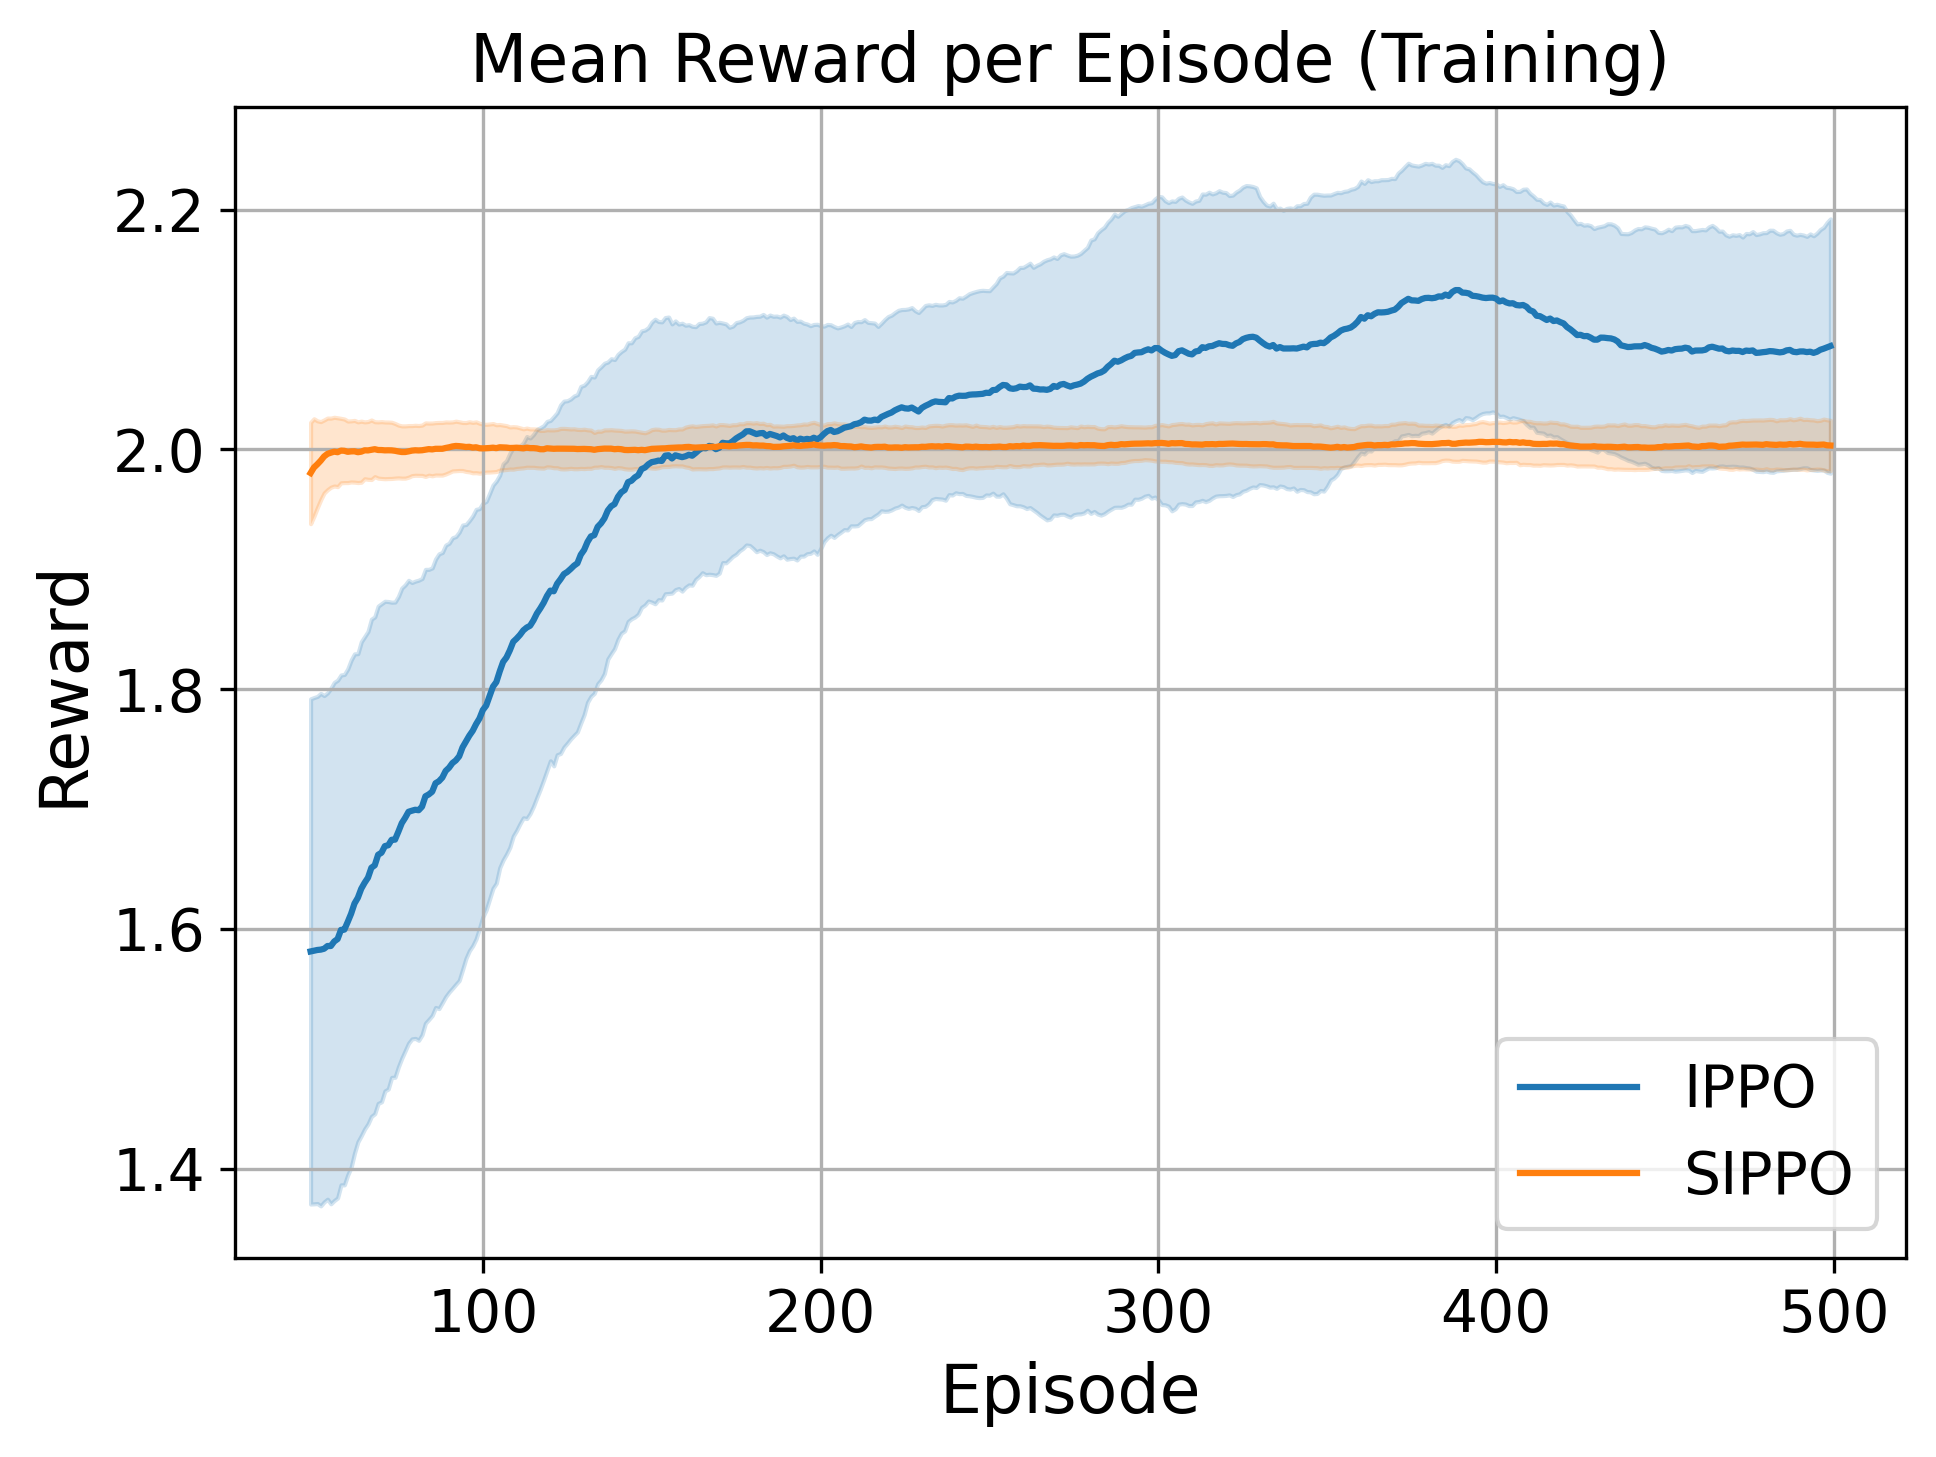
\includegraphics[width=0.9\textwidth]{Experiments/images/epgg/training_mu0_5_epgg.png}
        \vspace{0.3em}

        \textbf{(a)} Training ($\mu=0.5$)
        \label{fig:epgg_results:sub1}
    \end{minipage}
    \hfill
    \begin{minipage}[b]{0.3\textwidth}
        \centering
        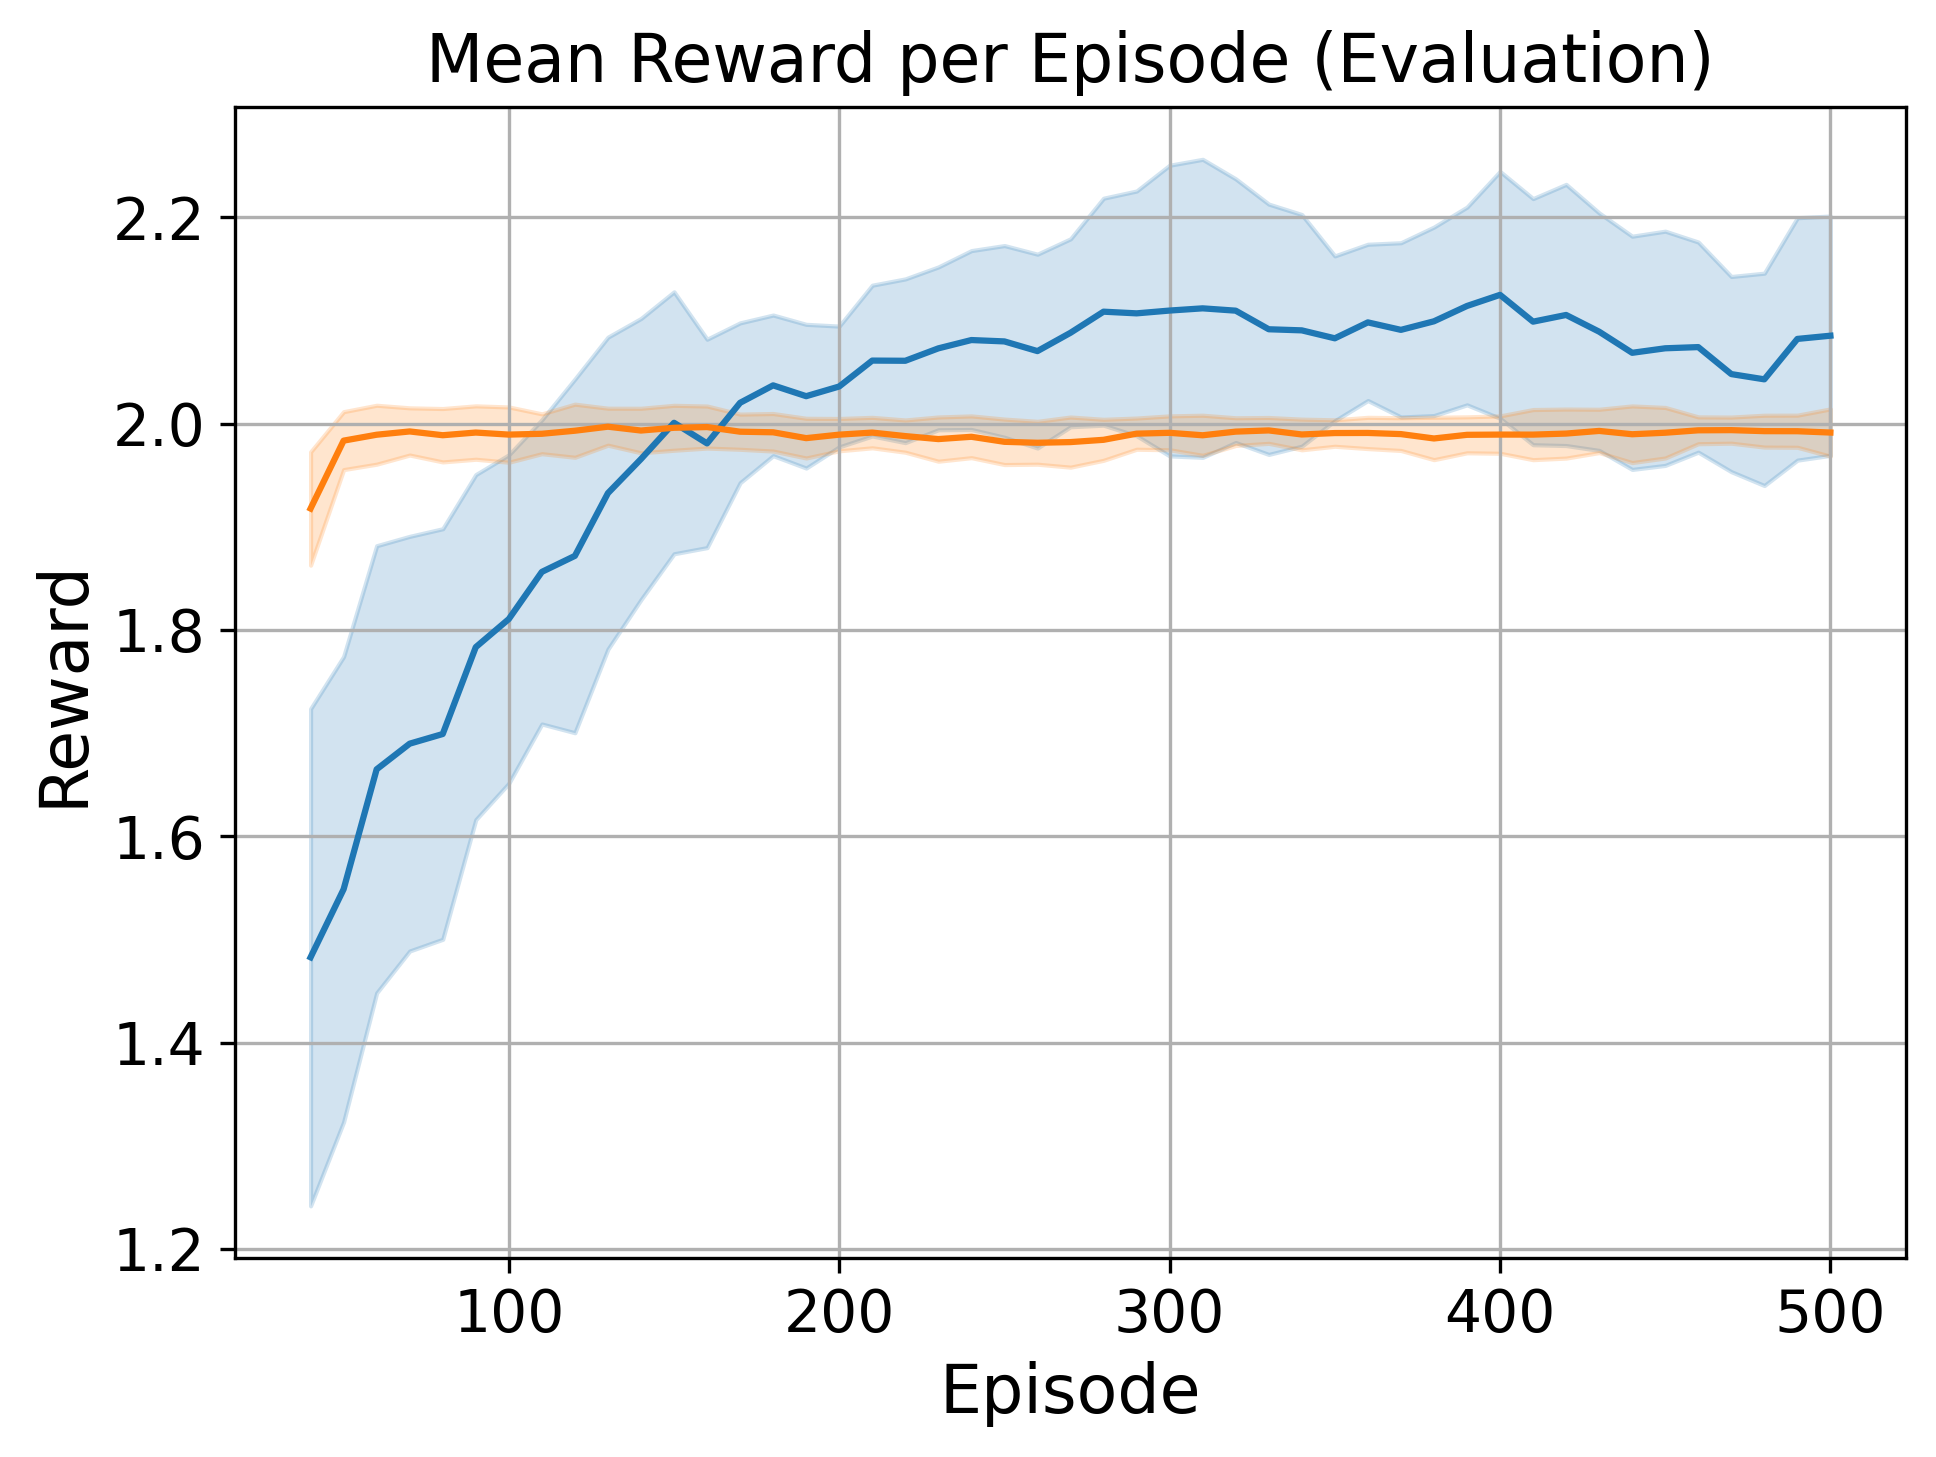
\includegraphics[width=0.9\textwidth]{Experiments/images/epgg/eval_mu0_5_epgg.png}
        \vspace{0.3em}

        \textbf{(b)} Evaluation ($\mu=0.5$)
        \label{fig:epgg_results:sub2}
    \end{minipage}
    \hfill
    \begin{minipage}[b]{0.3\textwidth}
        \centering
        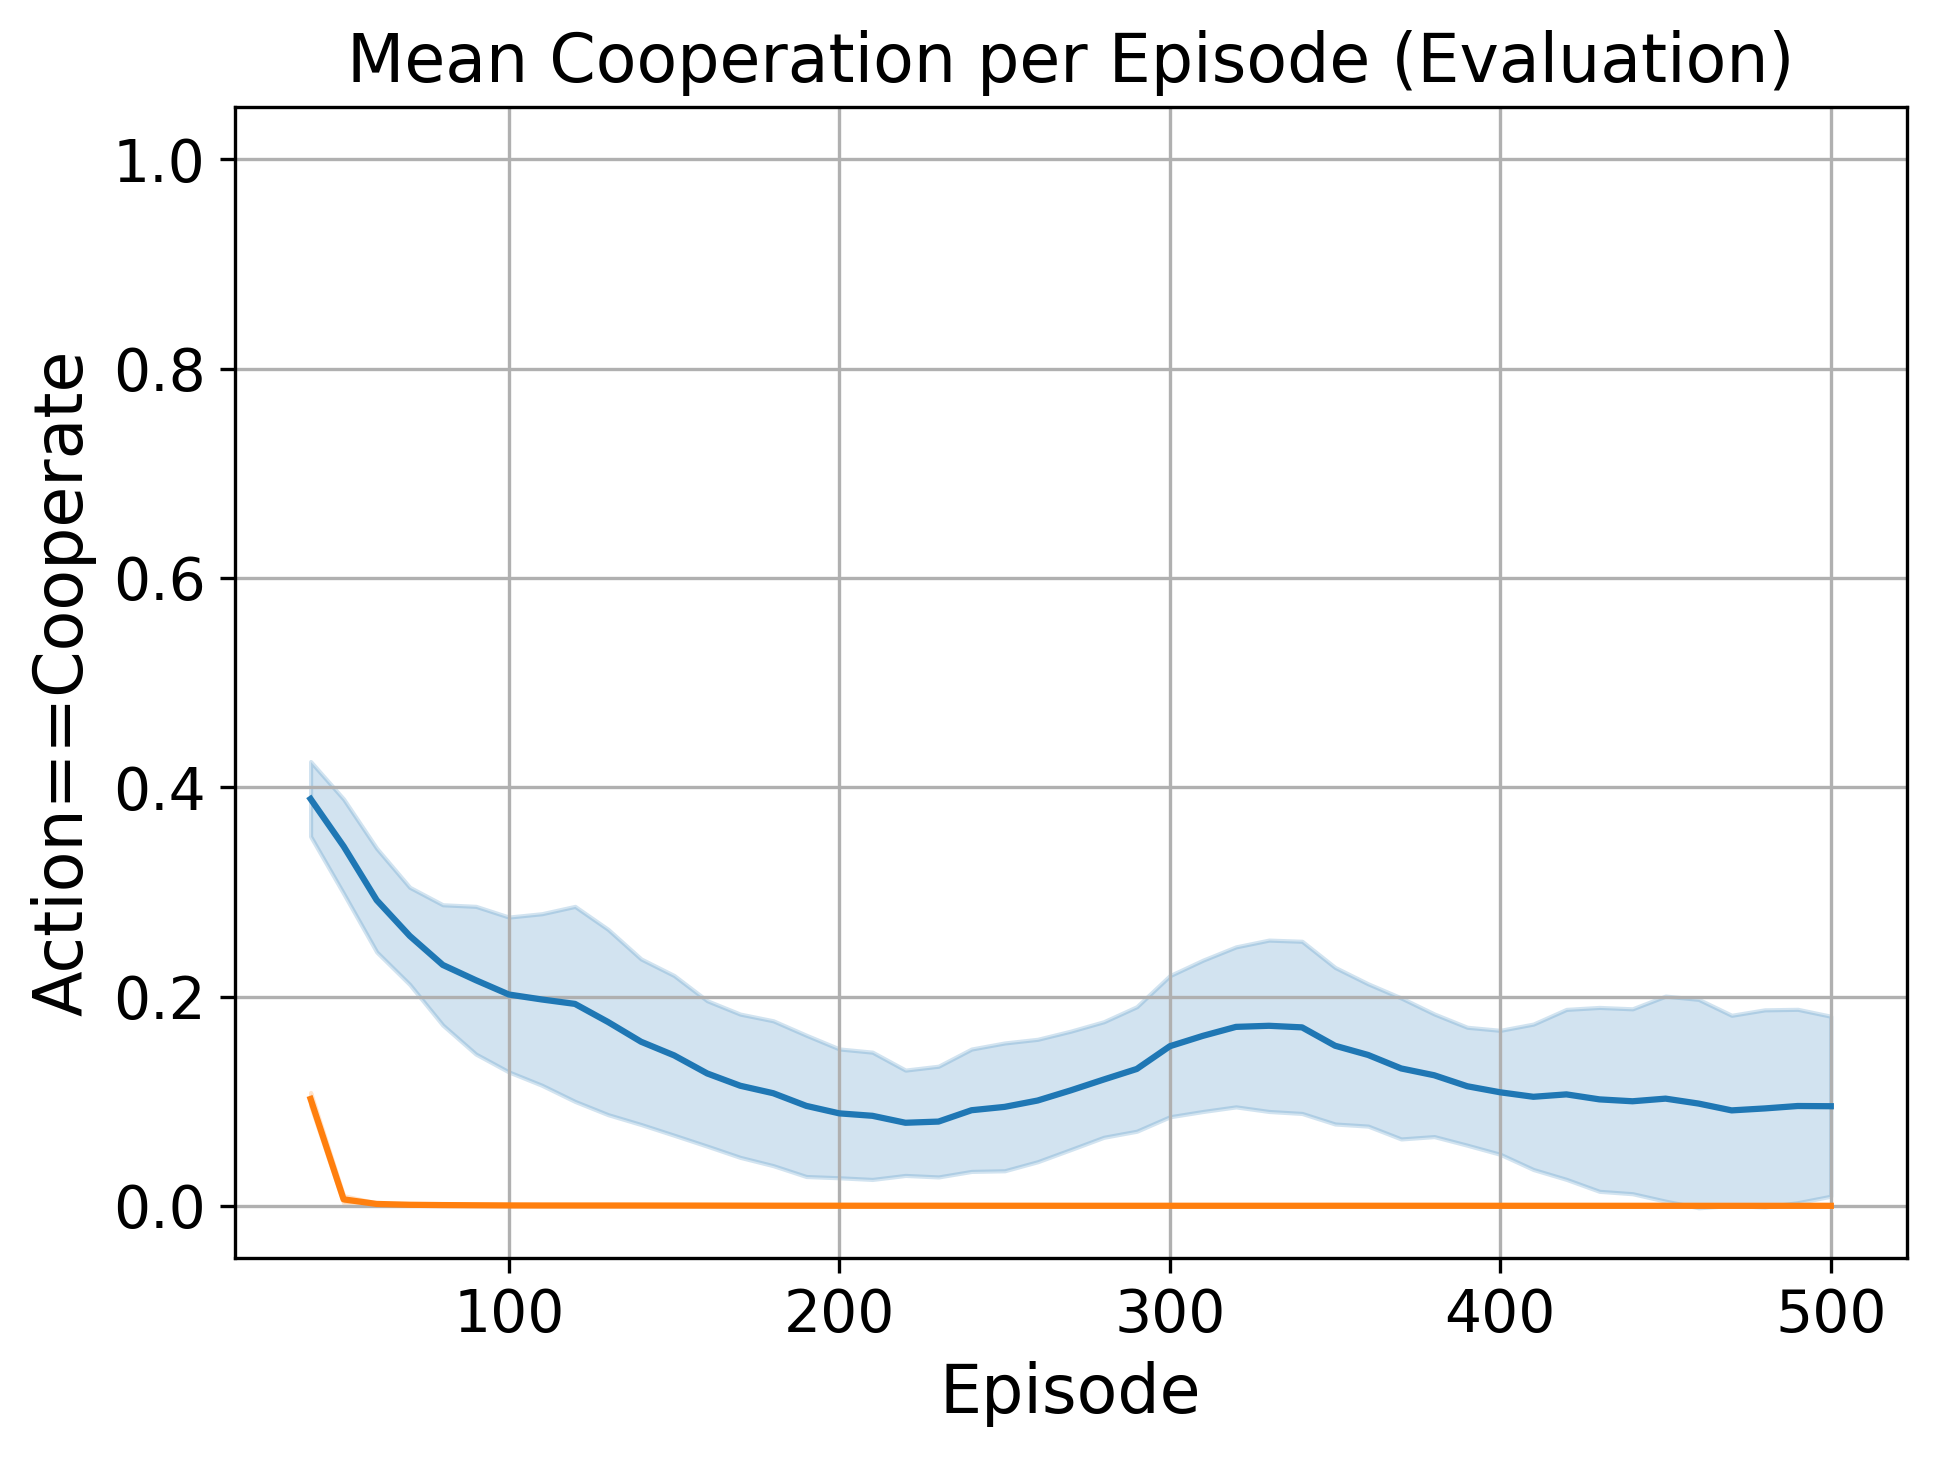
\includegraphics[width=0.9\textwidth]{Experiments/images/epgg/safety_mu0_5_epgg.png}
        \vspace{0.3em}

        \textbf{(c)} Safety ($\mu=0.5$)
        \label{fig:epgg_results:sub3}
    \end{minipage}

    \vspace{5pt}

    % Row 2: mu = 1.0
    \begin{minipage}[b]{0.3\textwidth}
        \centering
        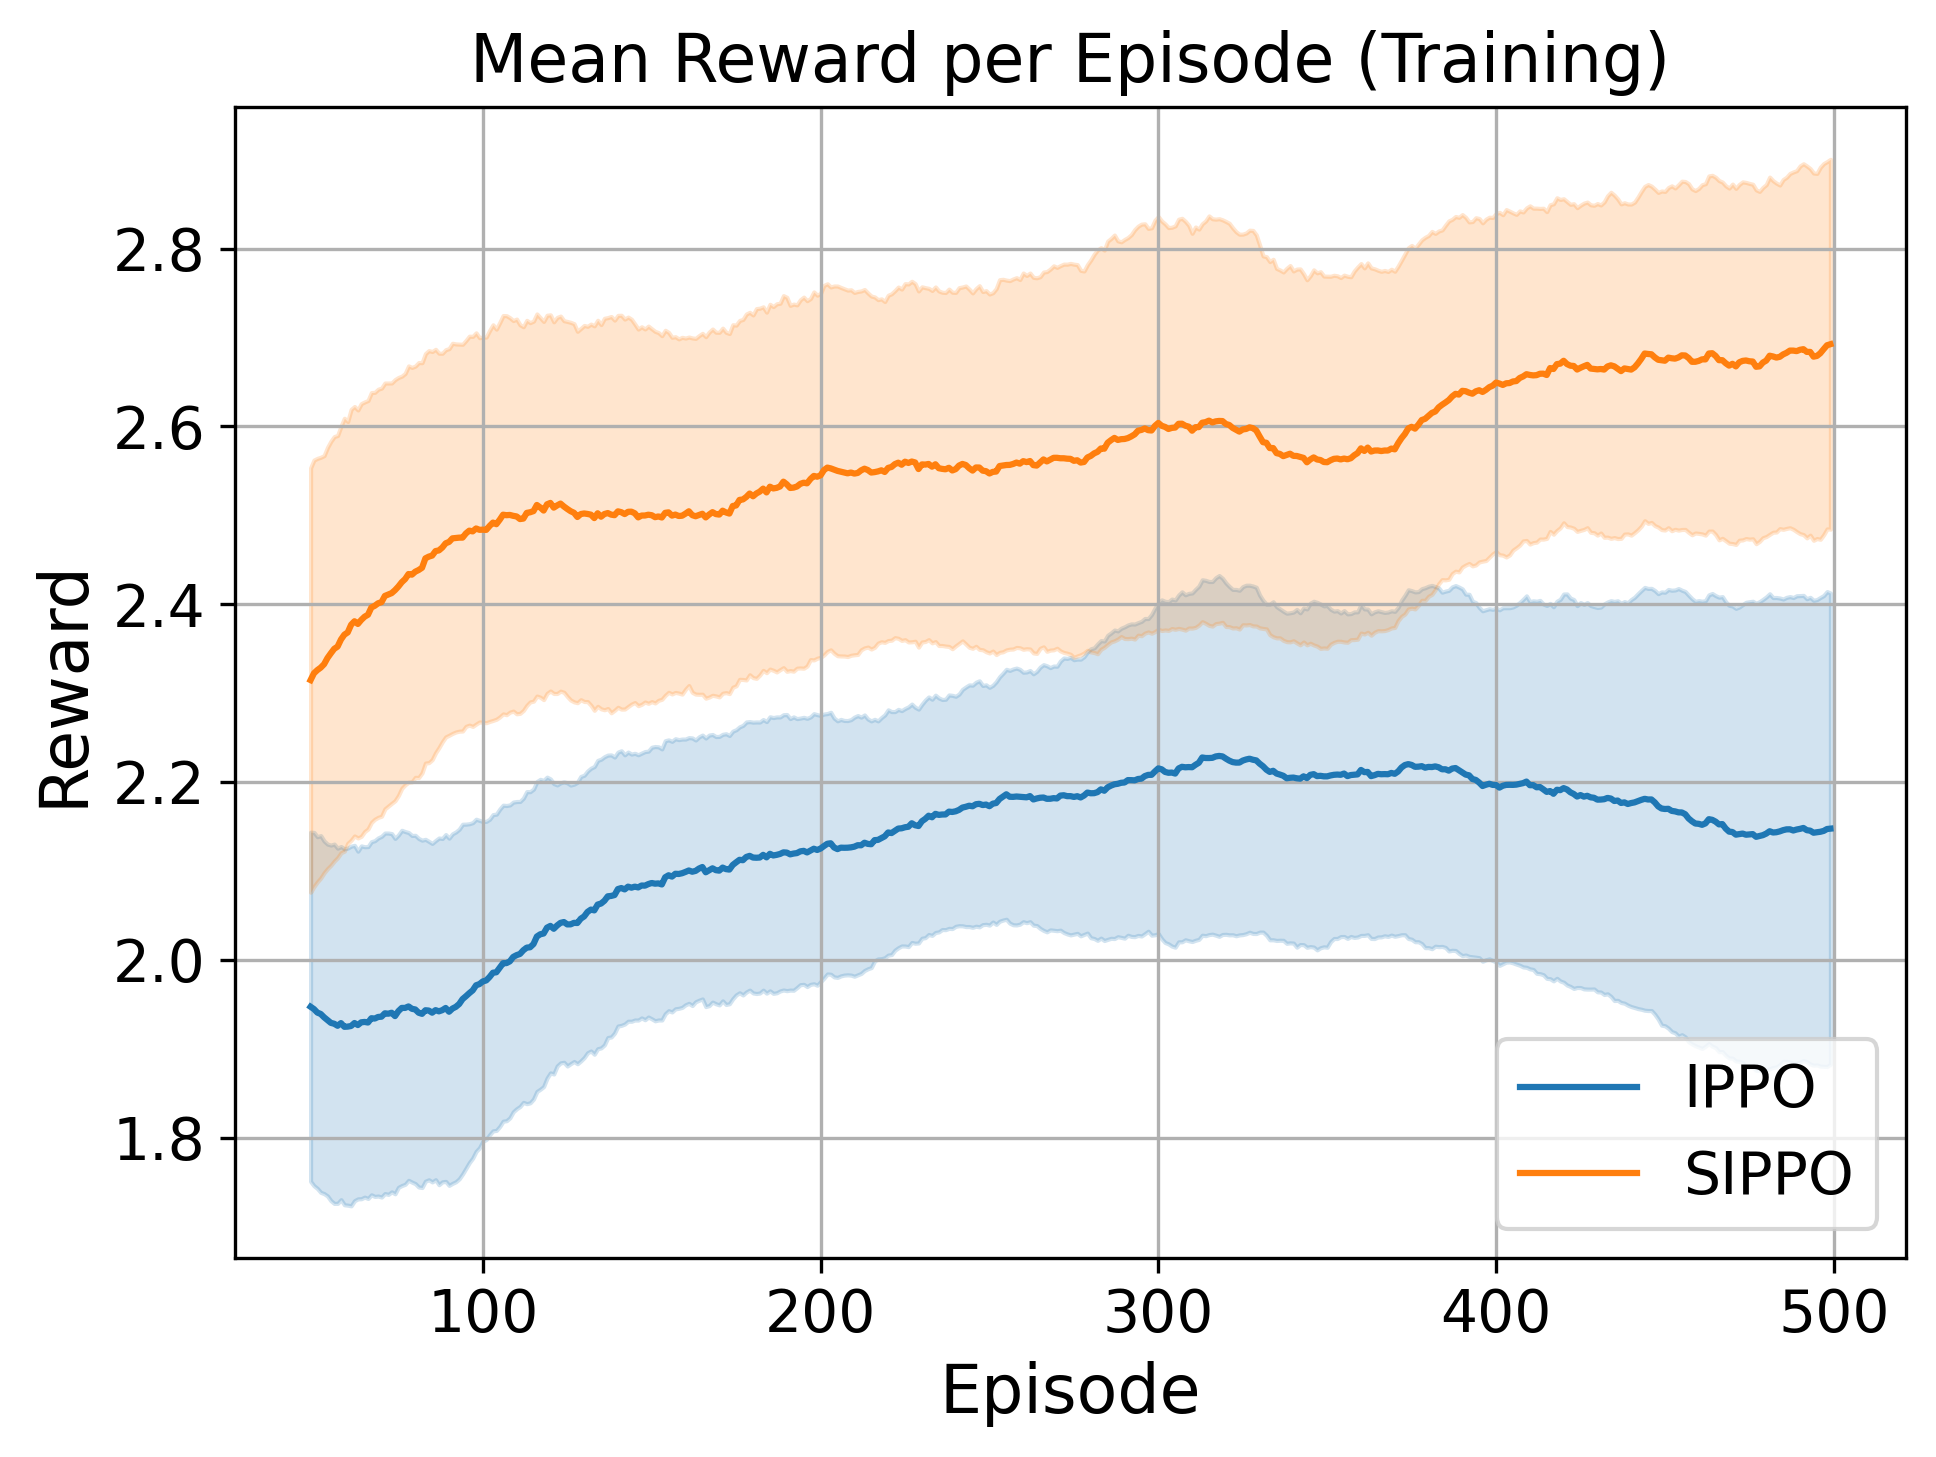
\includegraphics[width=0.9\textwidth]{Experiments/images/epgg/training_mu1_epgg.png}
        \vspace{0.3em}

        \textbf{(d)} Training ($\mu=1.0$)
        \label{fig:epgg_results:sub4}
    \end{minipage}
    \hfill
    \begin{minipage}[b]{0.3\textwidth}
        \centering
        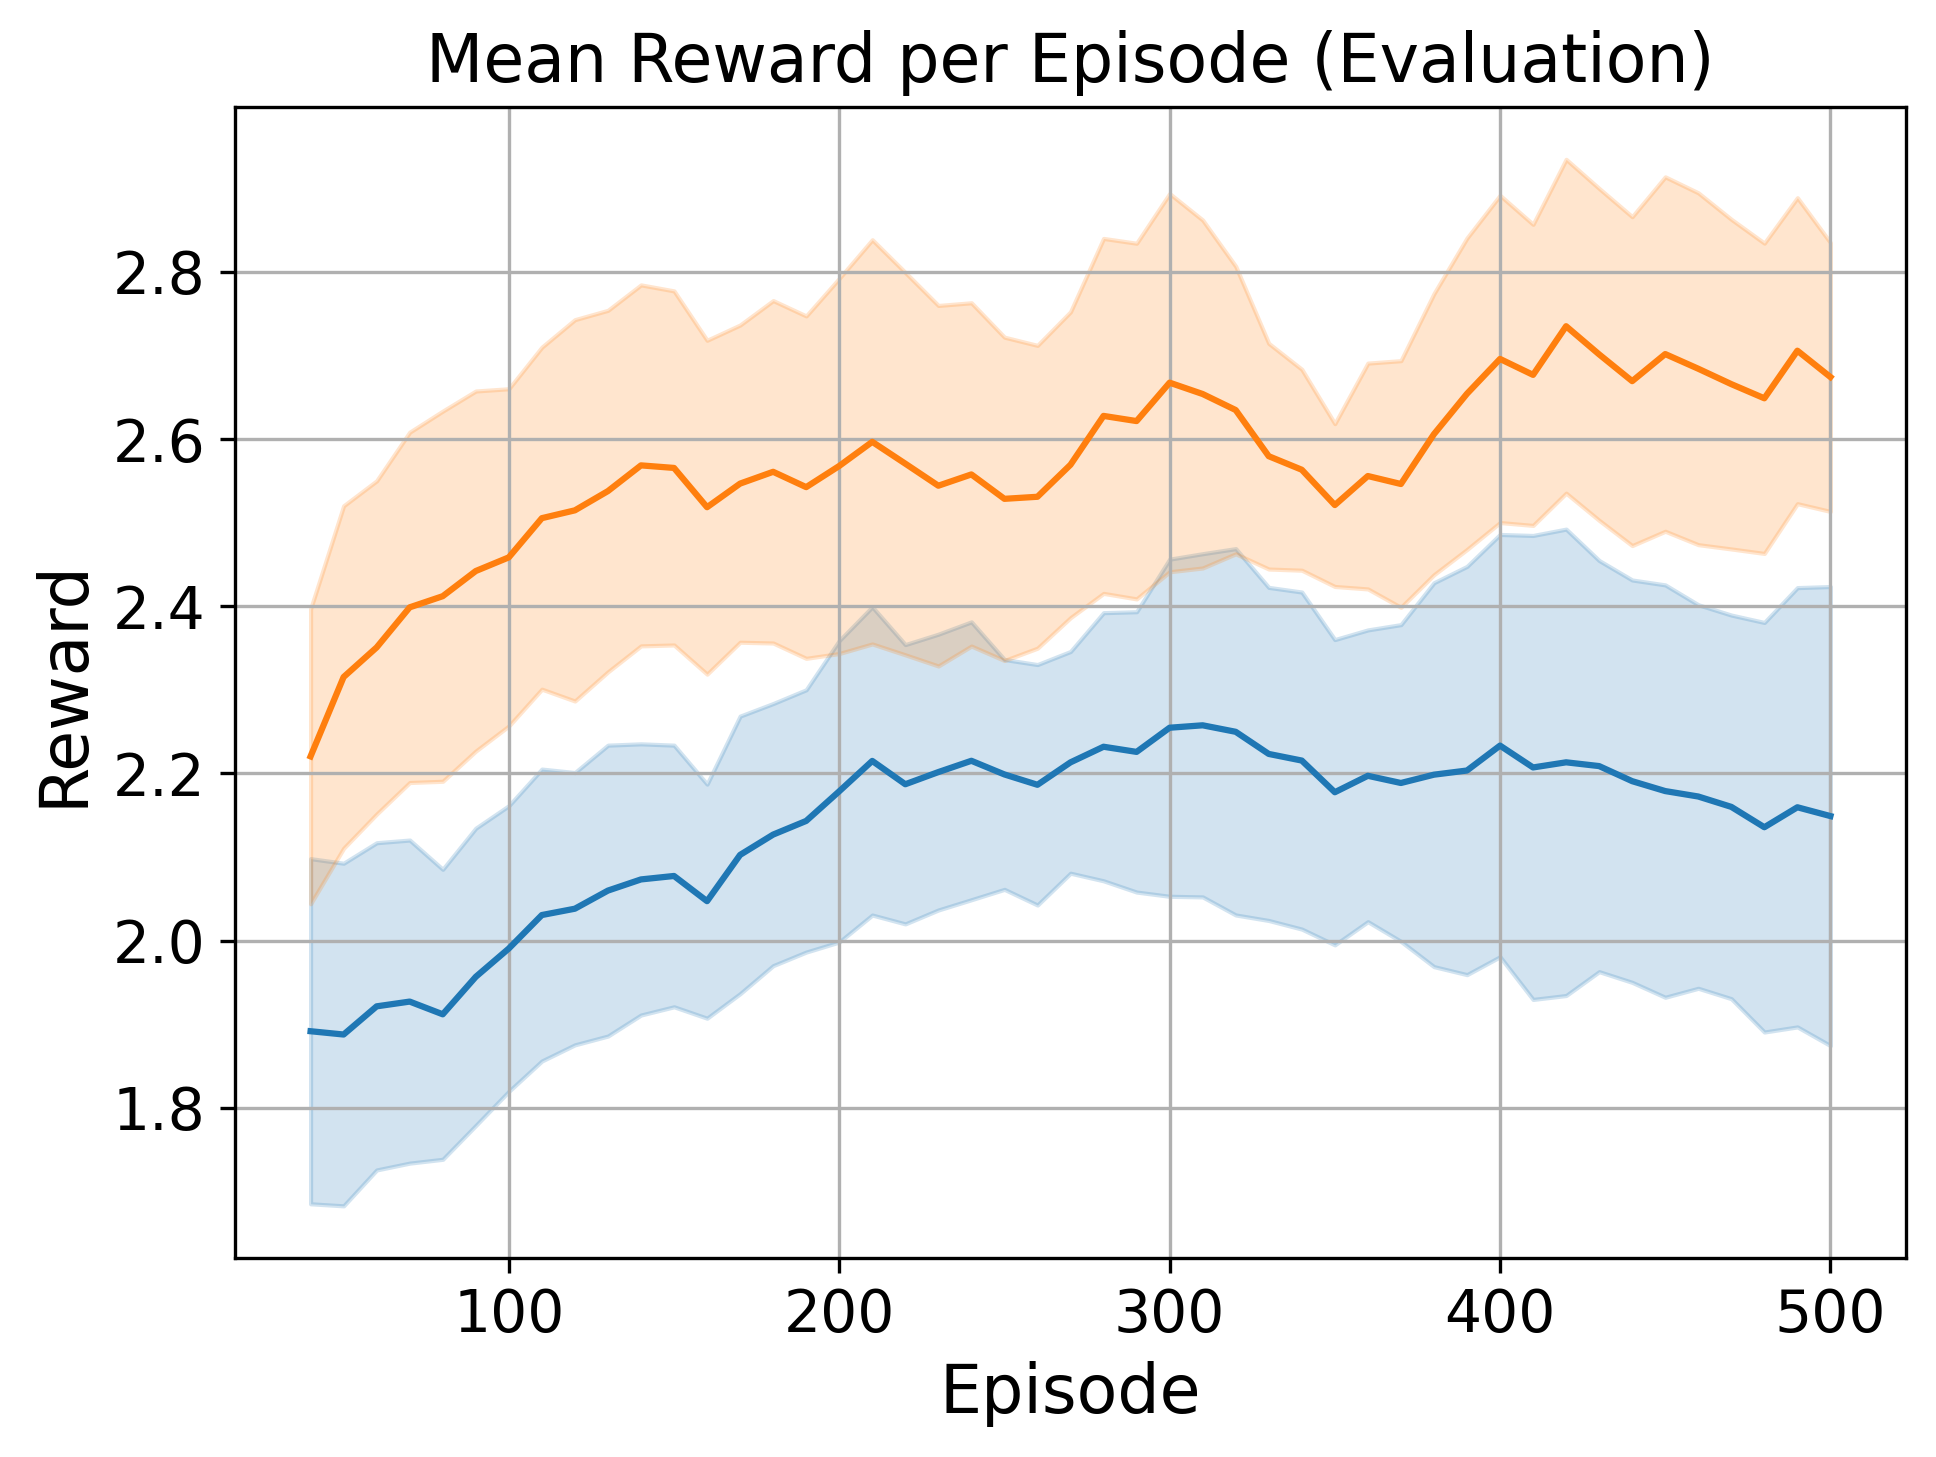
\includegraphics[width=0.9\textwidth]{Experiments/images/epgg/eval_mu1_epgg.png}
        \vspace{0.3em}

        \textbf{(e)} Evaluation ($\mu=1.0$)
        \label{fig:epgg_results:sub5}
    \end{minipage}
    \hfill
    \begin{minipage}[b]{0.3\textwidth}
        \centering
        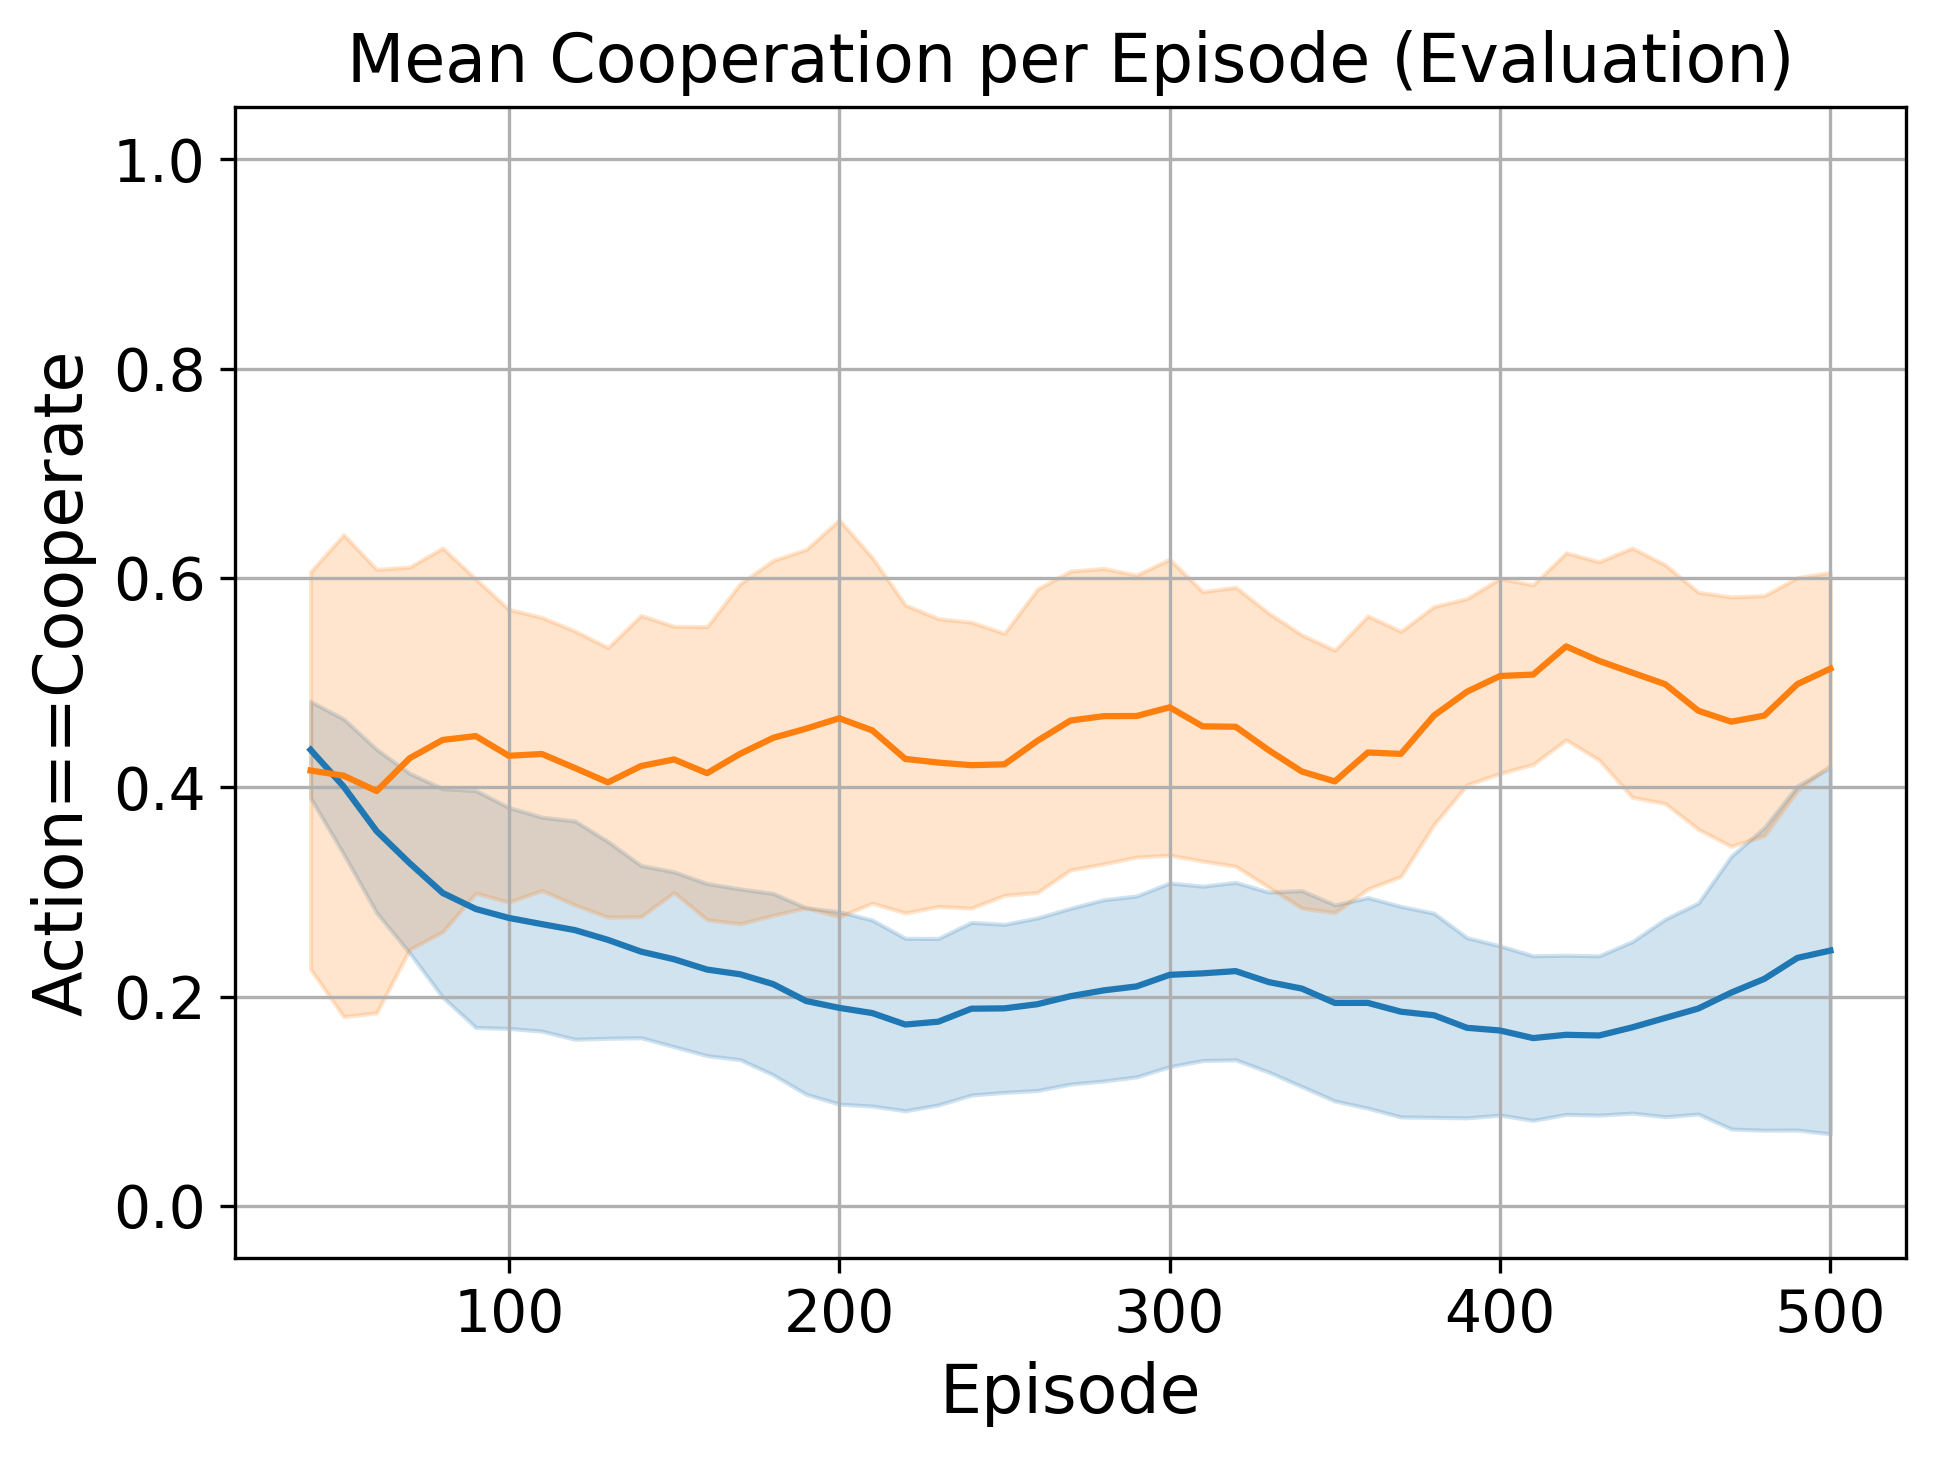
\includegraphics[width=0.9\textwidth]{Experiments/images/epgg/safety_mu1_epgg.png}
        \vspace{0.3em}

        \textbf{(f)} Safety ($\mu=1.0$)
        \label{fig:epgg_results:sub6}
    \end{minipage}

    \vspace{5pt}

    % Row 3: mu = 1.5
    \begin{minipage}[b]{0.3\textwidth}
        \centering
        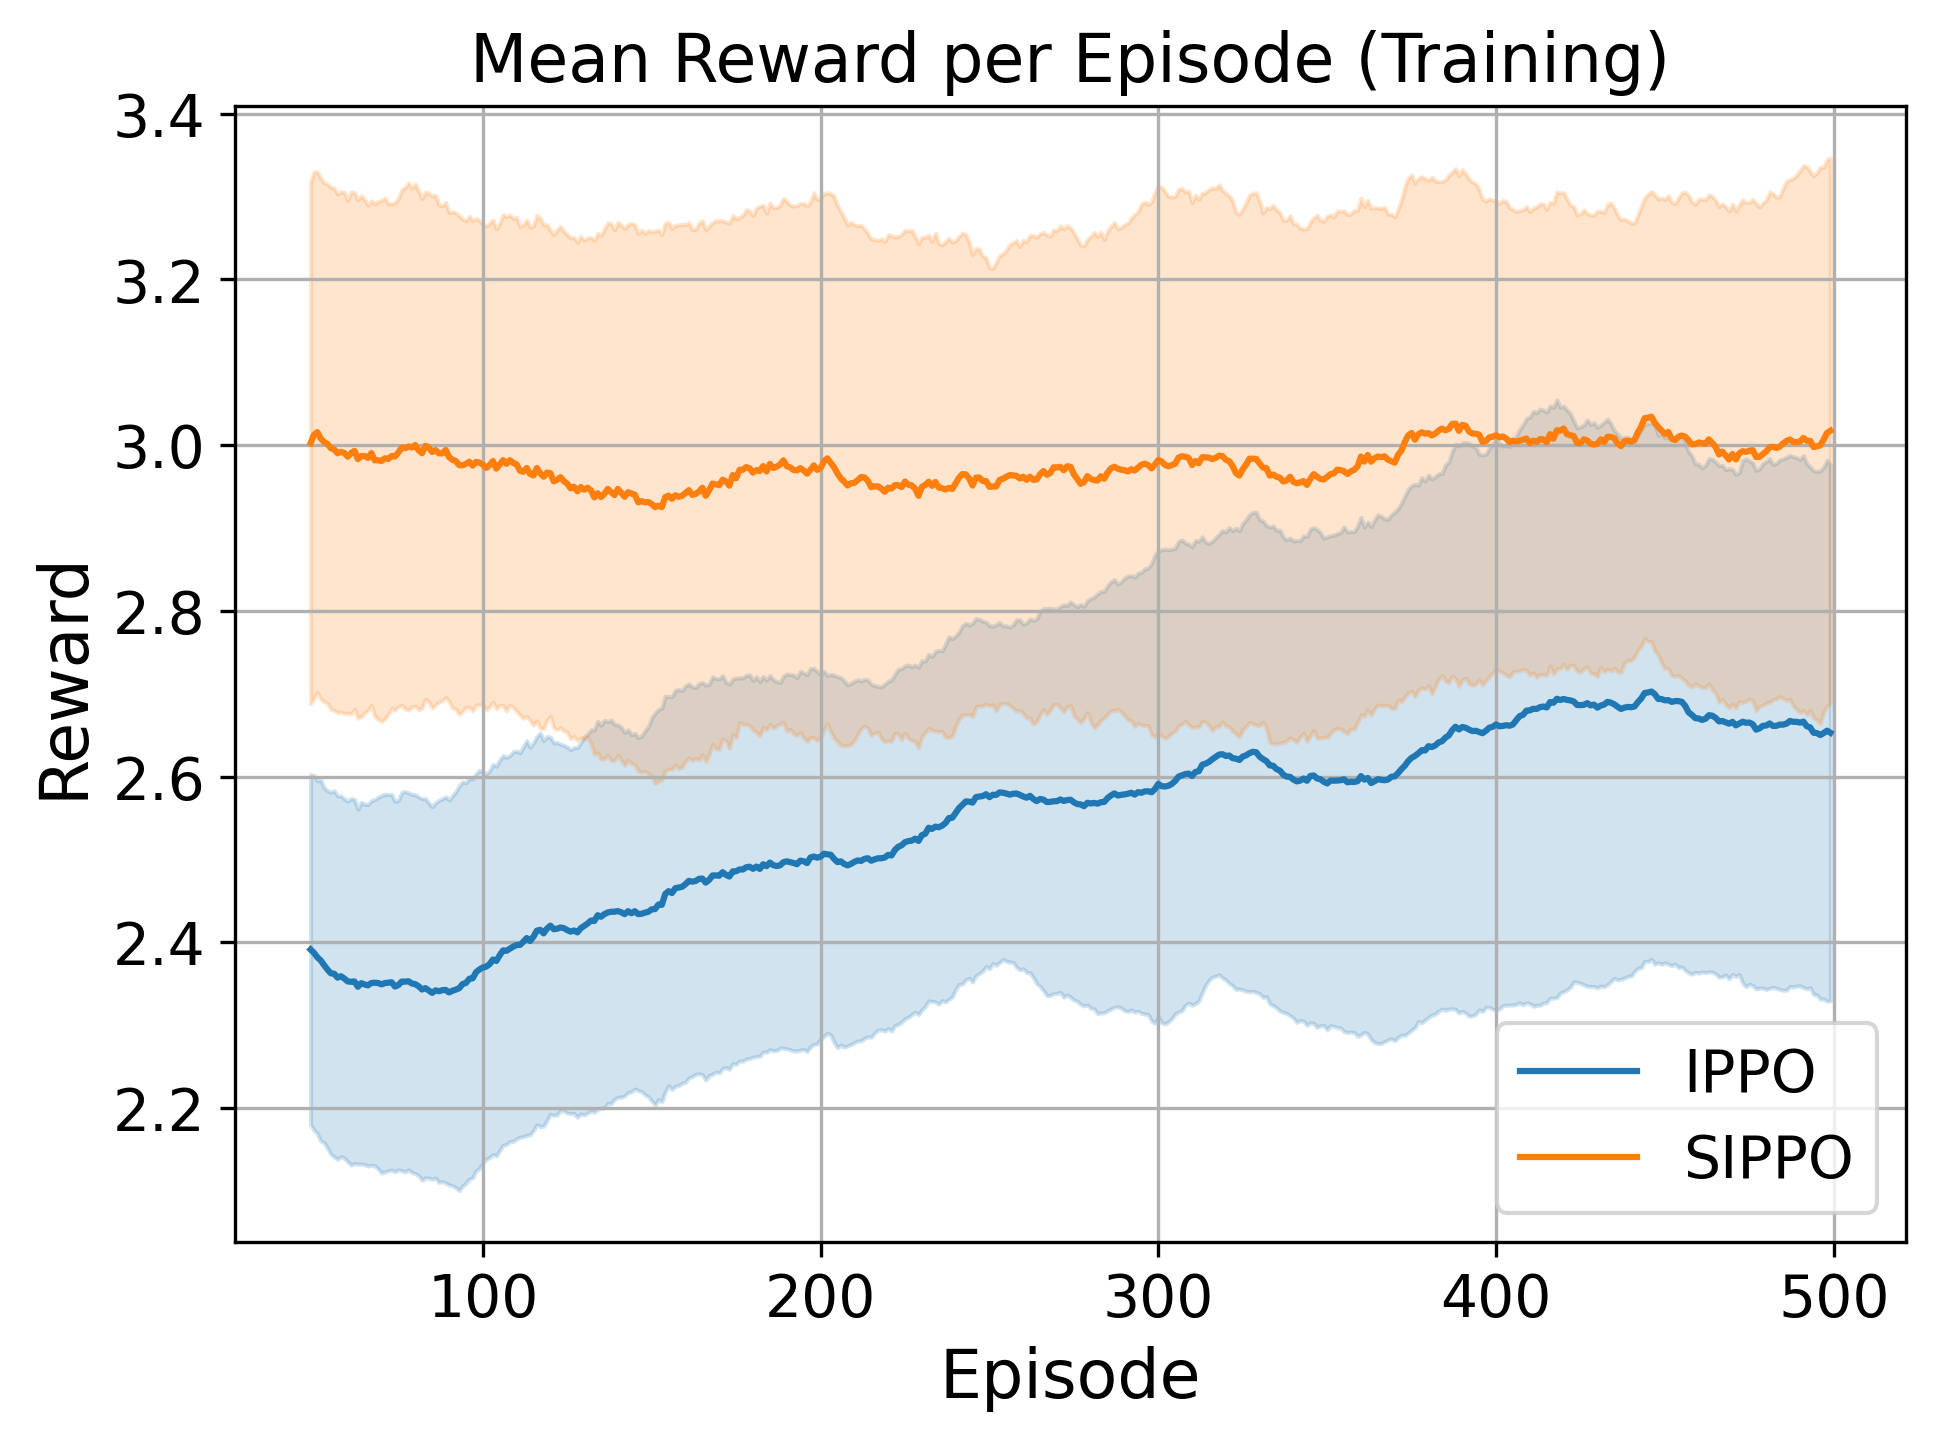
\includegraphics[width=0.9\textwidth]{Experiments/images/epgg/training_mu1_5_epgg.png}
        \vspace{0.3em}

        \textbf{(g)} Training ($\mu=1.5$)
        \label{fig:epgg_results:sub7}
    \end{minipage}
    \hfill
    \begin{minipage}[b]{0.3\textwidth}
        \centering
        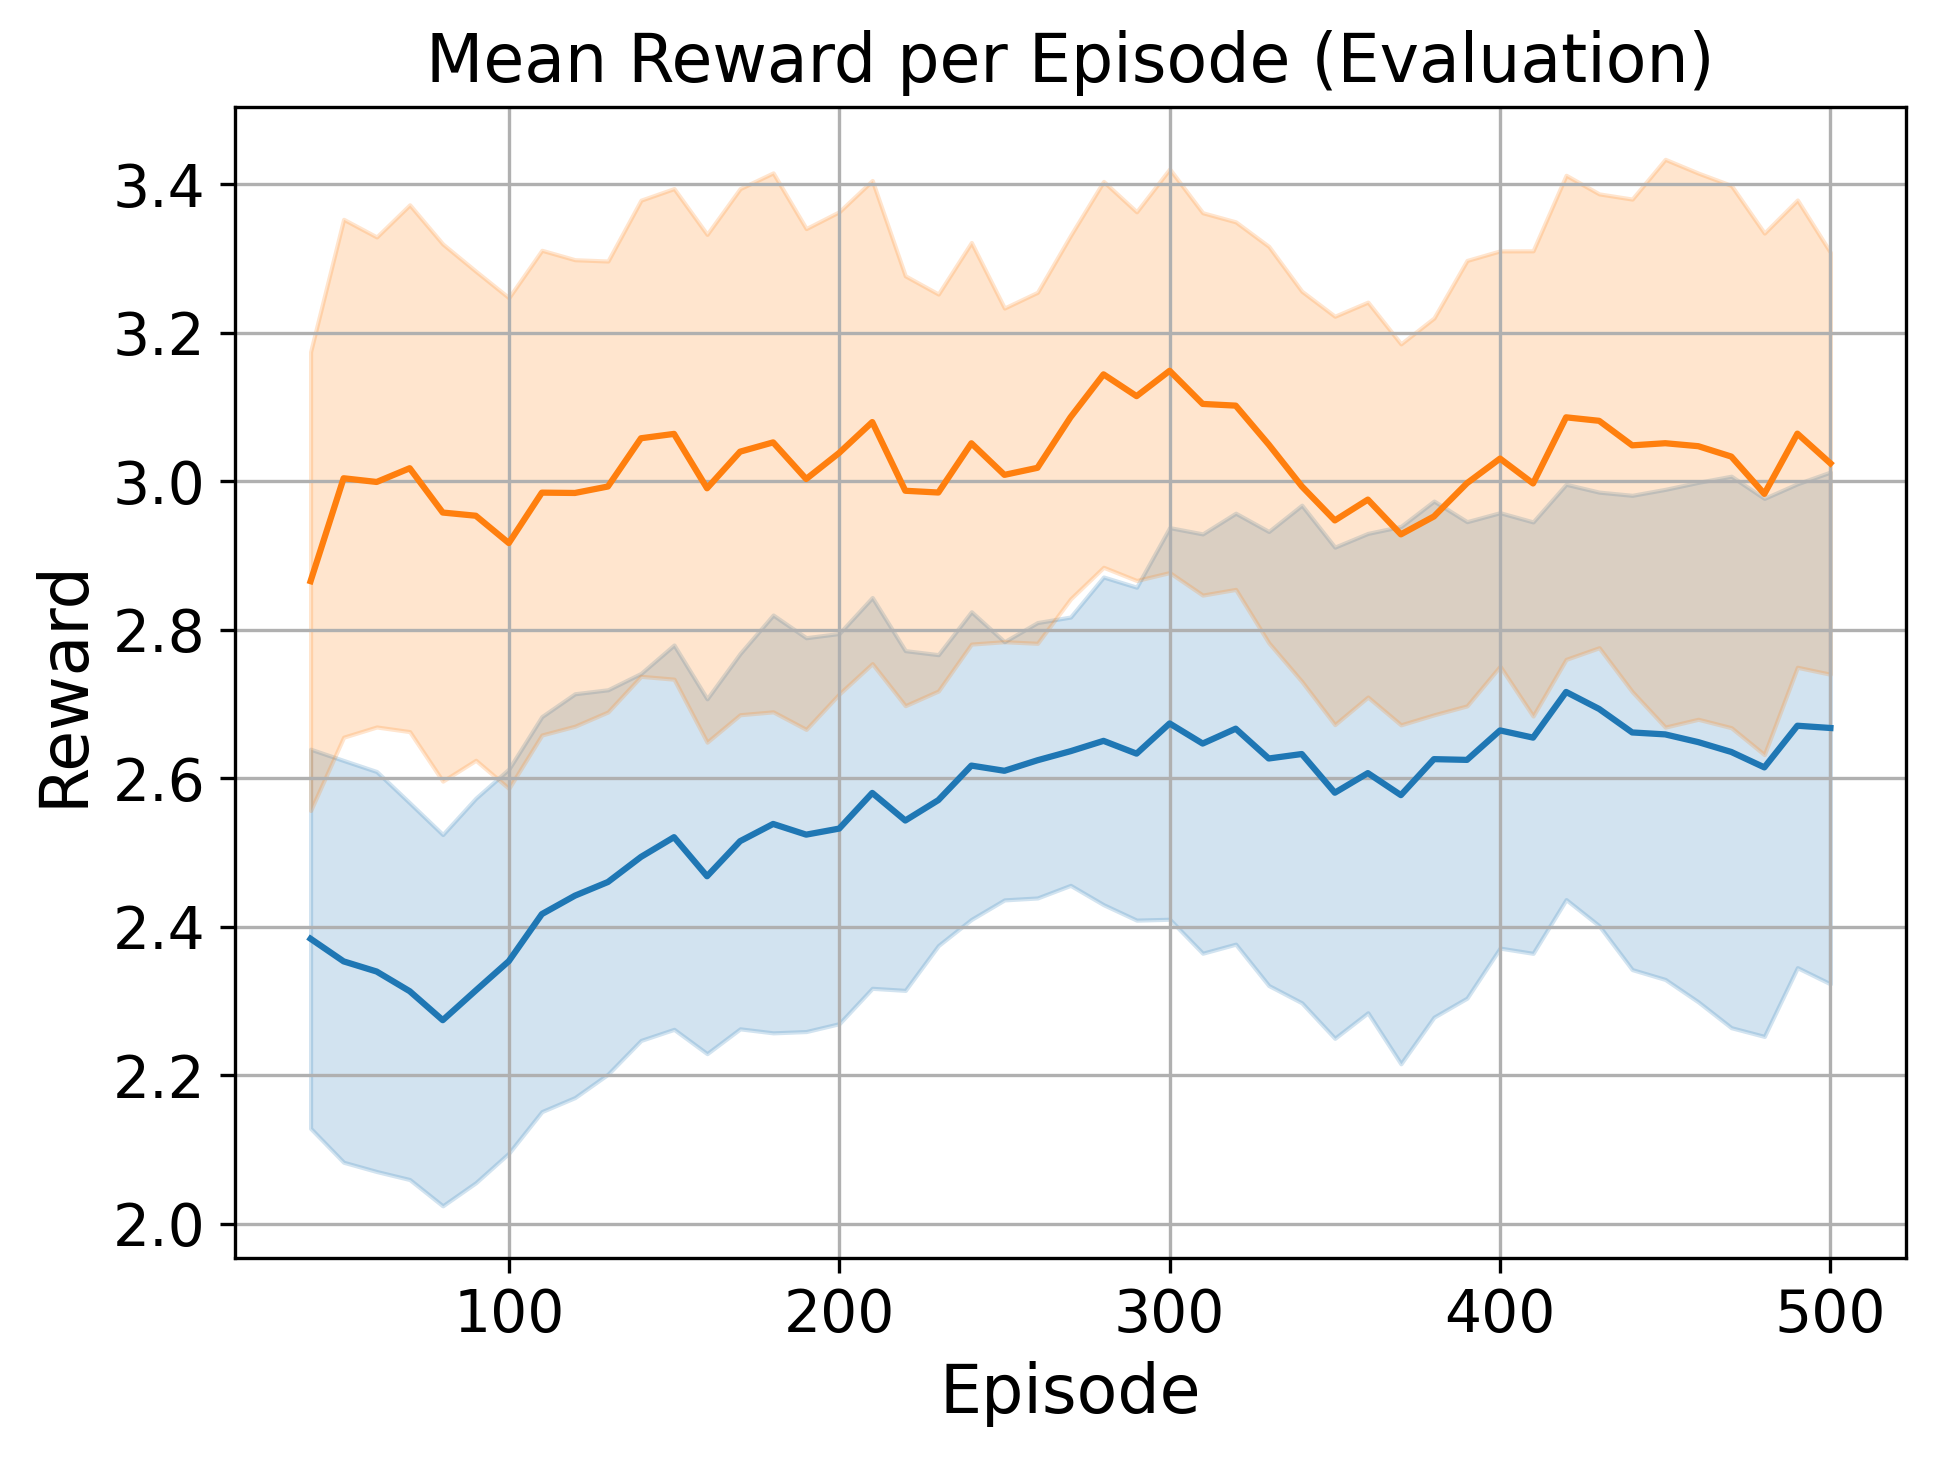
\includegraphics[width=0.9\textwidth]{Experiments/images/epgg/eval_mu1_5_epgg.png}
        \vspace{0.3em}

        \textbf{(h)} Evaluation ($\mu=1.5$)
        \label{fig:epgg_results:sub8}
    \end{minipage}
    \hfill
    \begin{minipage}[b]{0.3\textwidth}
        \centering
        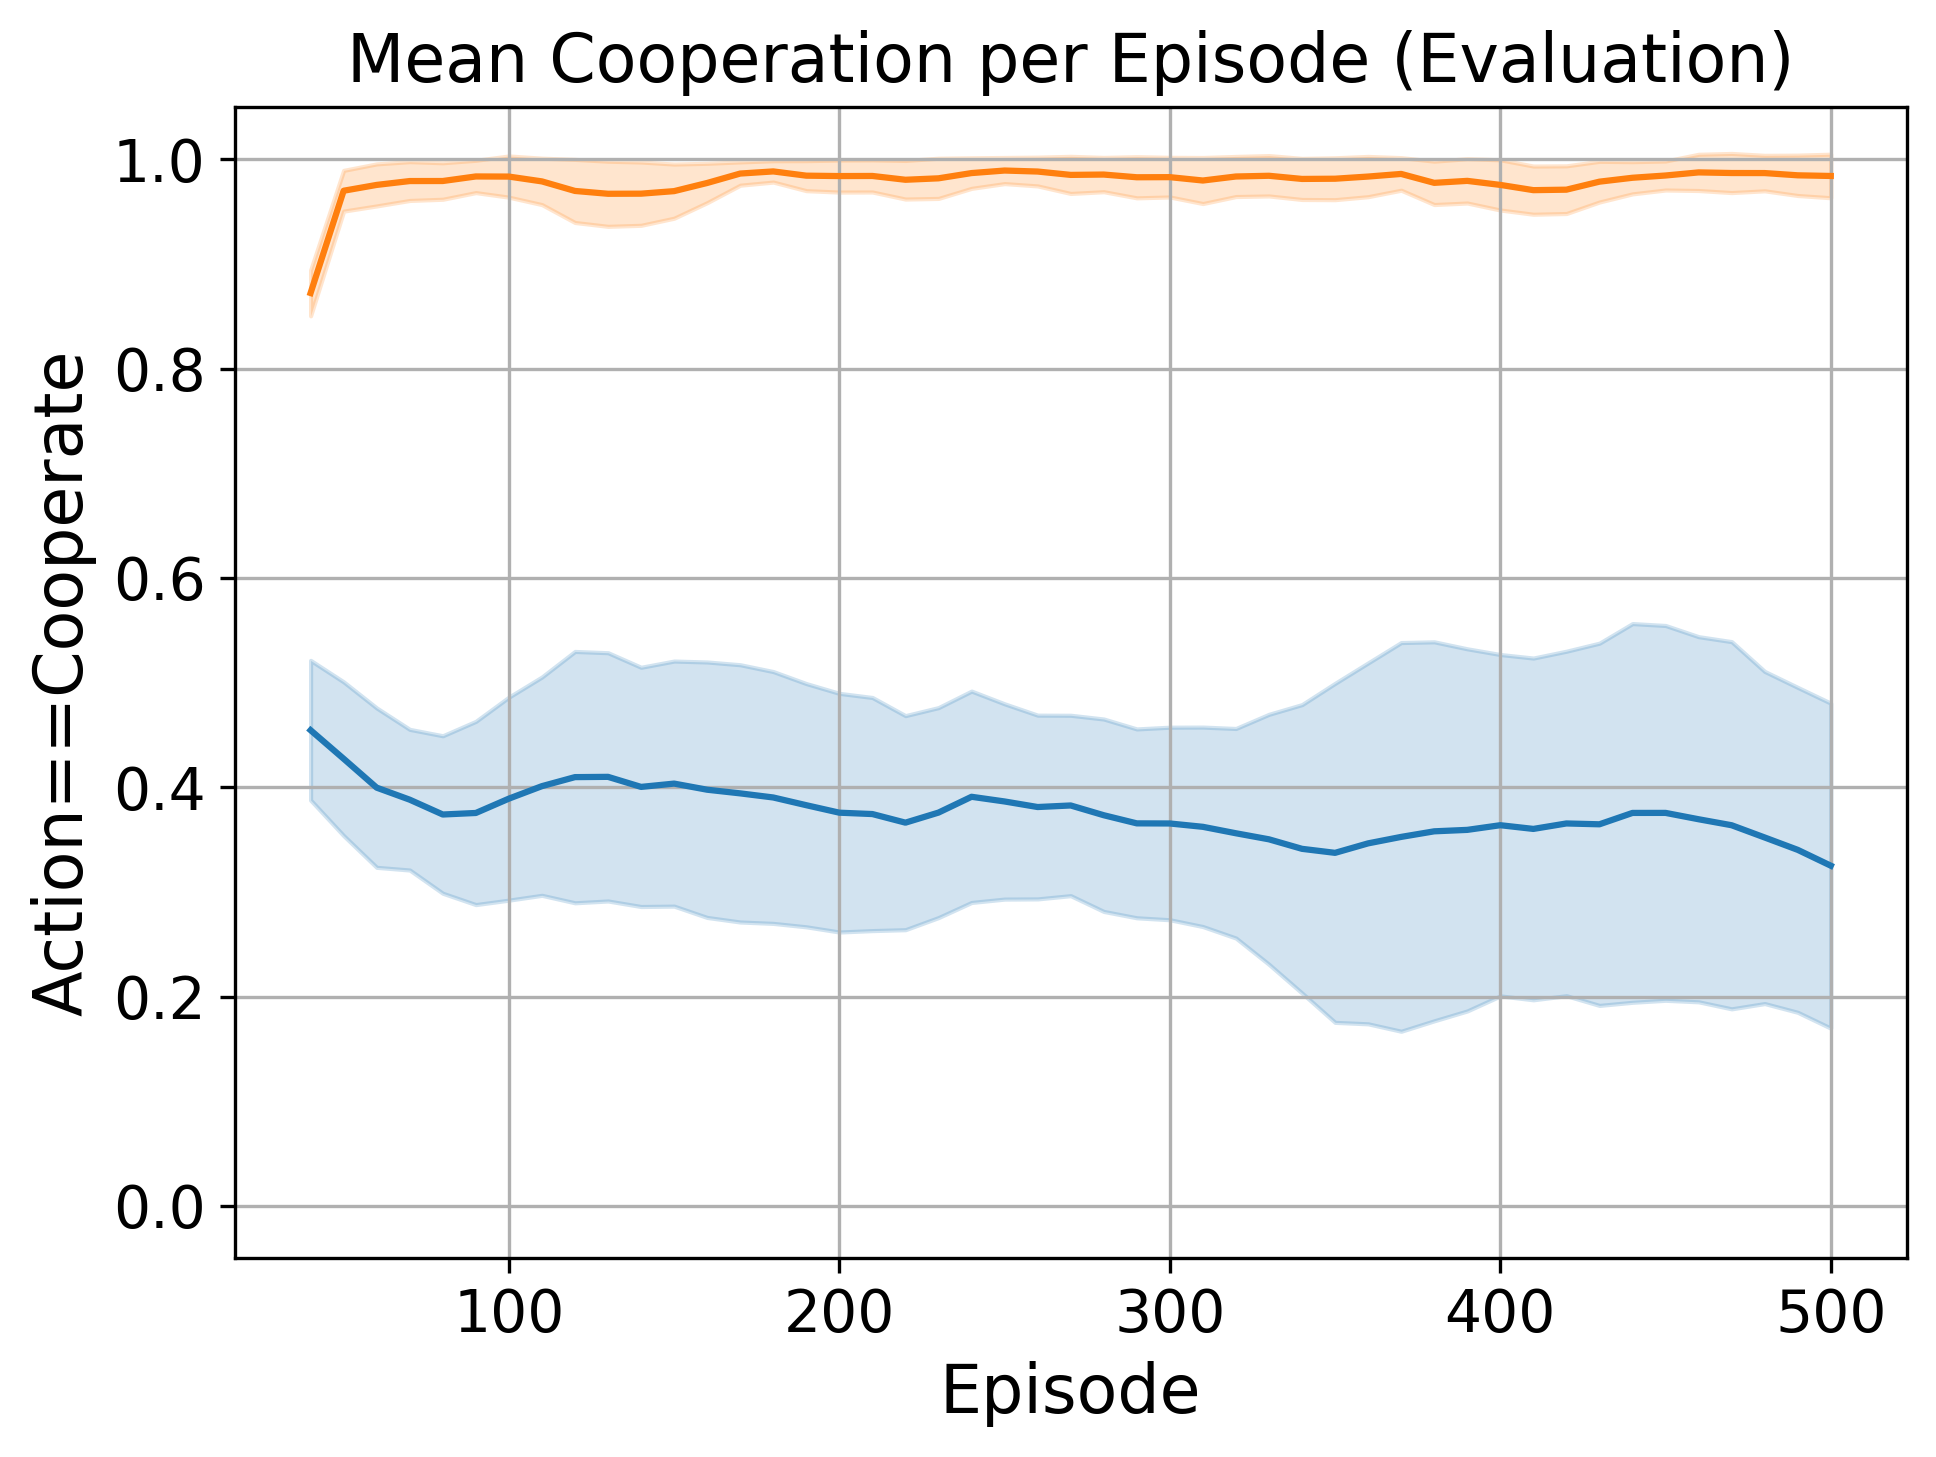
\includegraphics[width=0.9\textwidth]{Experiments/images/epgg/safety_mu1_5_epgg.png}
        \vspace{0.3em}

        \textbf{(i)} Safety ($\mu=1.5$)
        \label{fig:epgg_results:sub9}
    \end{minipage}

    \vspace{5pt}

    % Row 4: mu = 2.5
    \begin{minipage}[b]{0.3\textwidth}
        \centering
        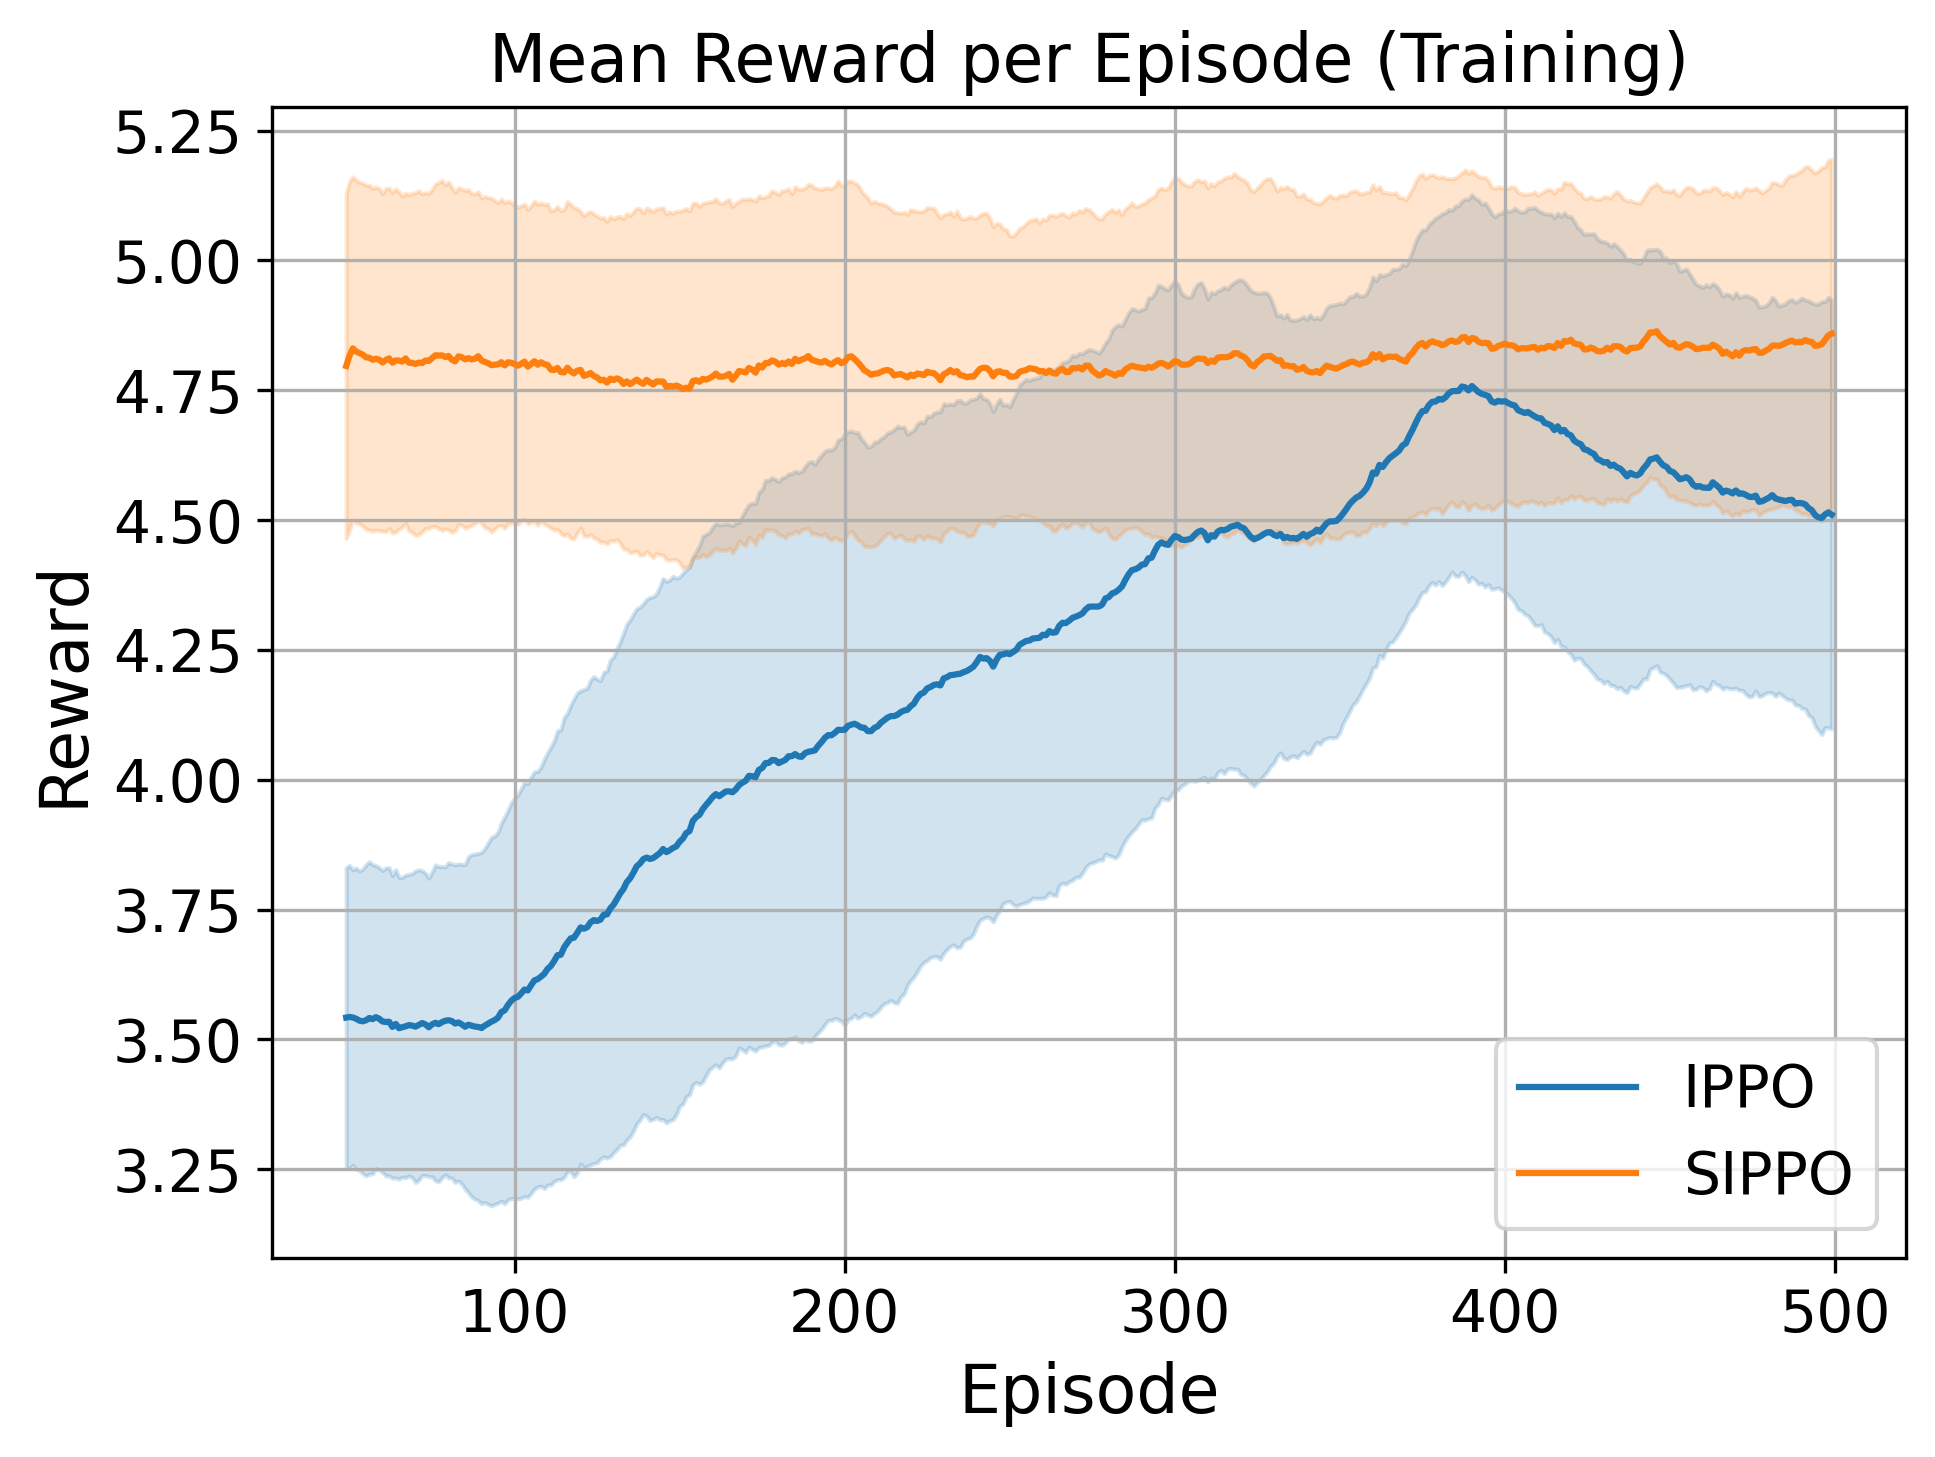
\includegraphics[width=0.9\textwidth]{Experiments/images/epgg/training_mu2_5_epgg.png}
        \vspace{0.3em}

        \textbf{(j)} Training ($\mu=2.5$)
        \label{fig:epgg_results:sub10}
    \end{minipage}
    \hfill
    \begin{minipage}[b]{0.3\textwidth}
        \centering
        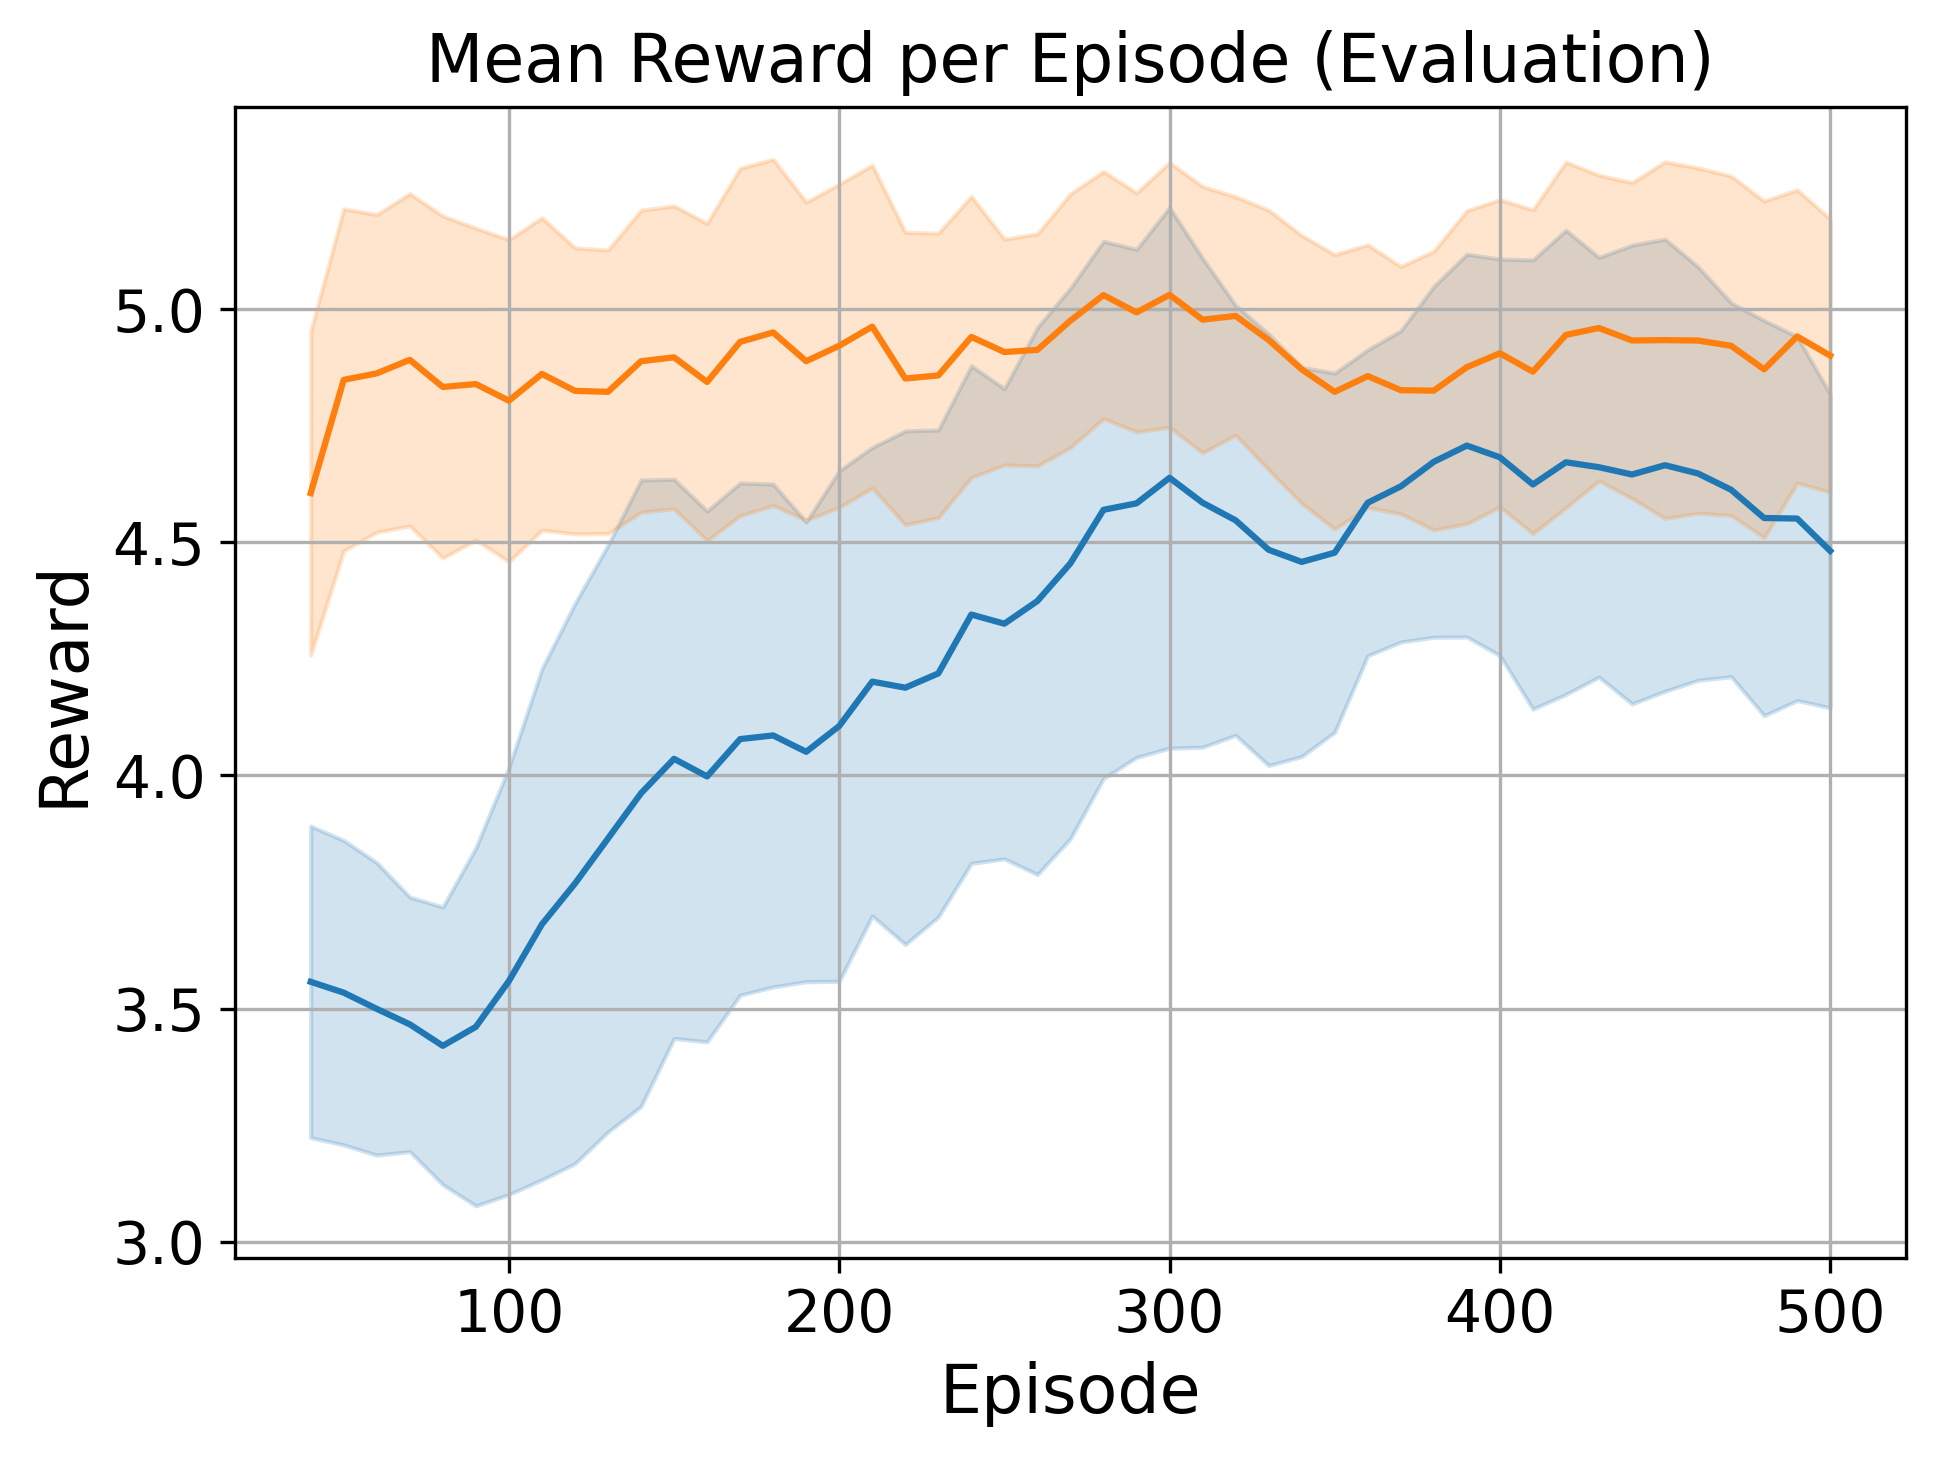
\includegraphics[width=0.9\textwidth]{Experiments/images/epgg/eval_mu2_5_epgg.png}
        \vspace{0.3em}

        \textbf{(k)} Evaluation ($\mu=2.5$)
        \label{fig:epgg_results:sub11}
    \end{minipage}
    \hfill
    \begin{minipage}[b]{0.3\textwidth}
        \centering
        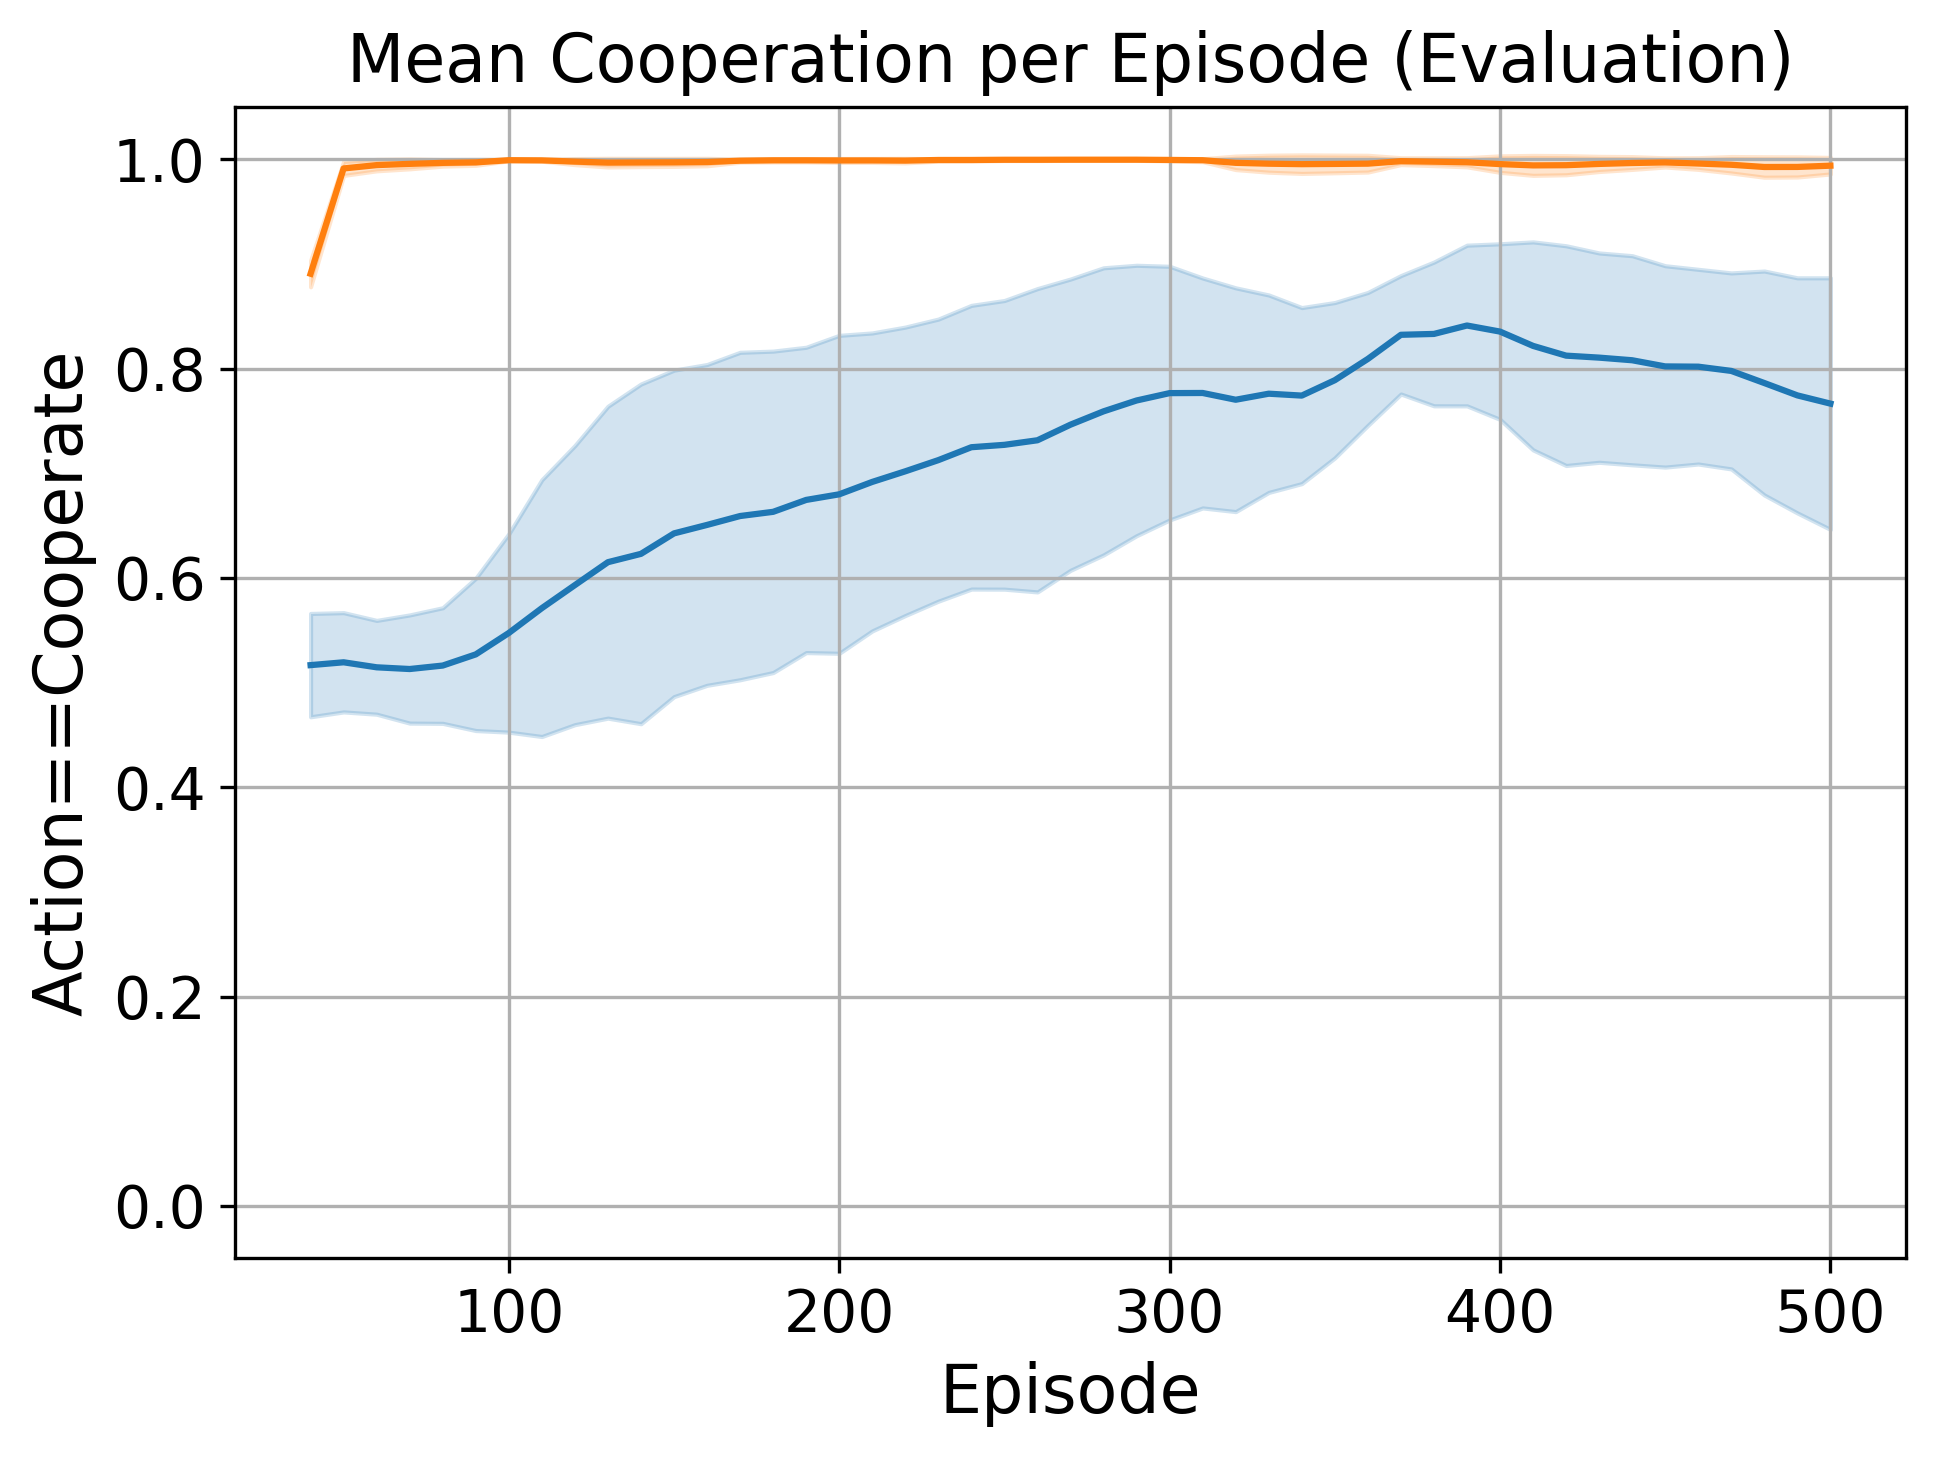
\includegraphics[width=0.9\textwidth]{Experiments/images/epgg/safety_mu2_5_epgg.png}
        \vspace{0.3em}

        \textbf{(l)} Safety ($\mu=2.5$)
        \label{fig:epgg_results:sub12}
    \end{minipage}

    \vspace{5pt}

    % Row 5: mu = 5.0
    \begin{minipage}[b]{0.3\textwidth}
        \centering
        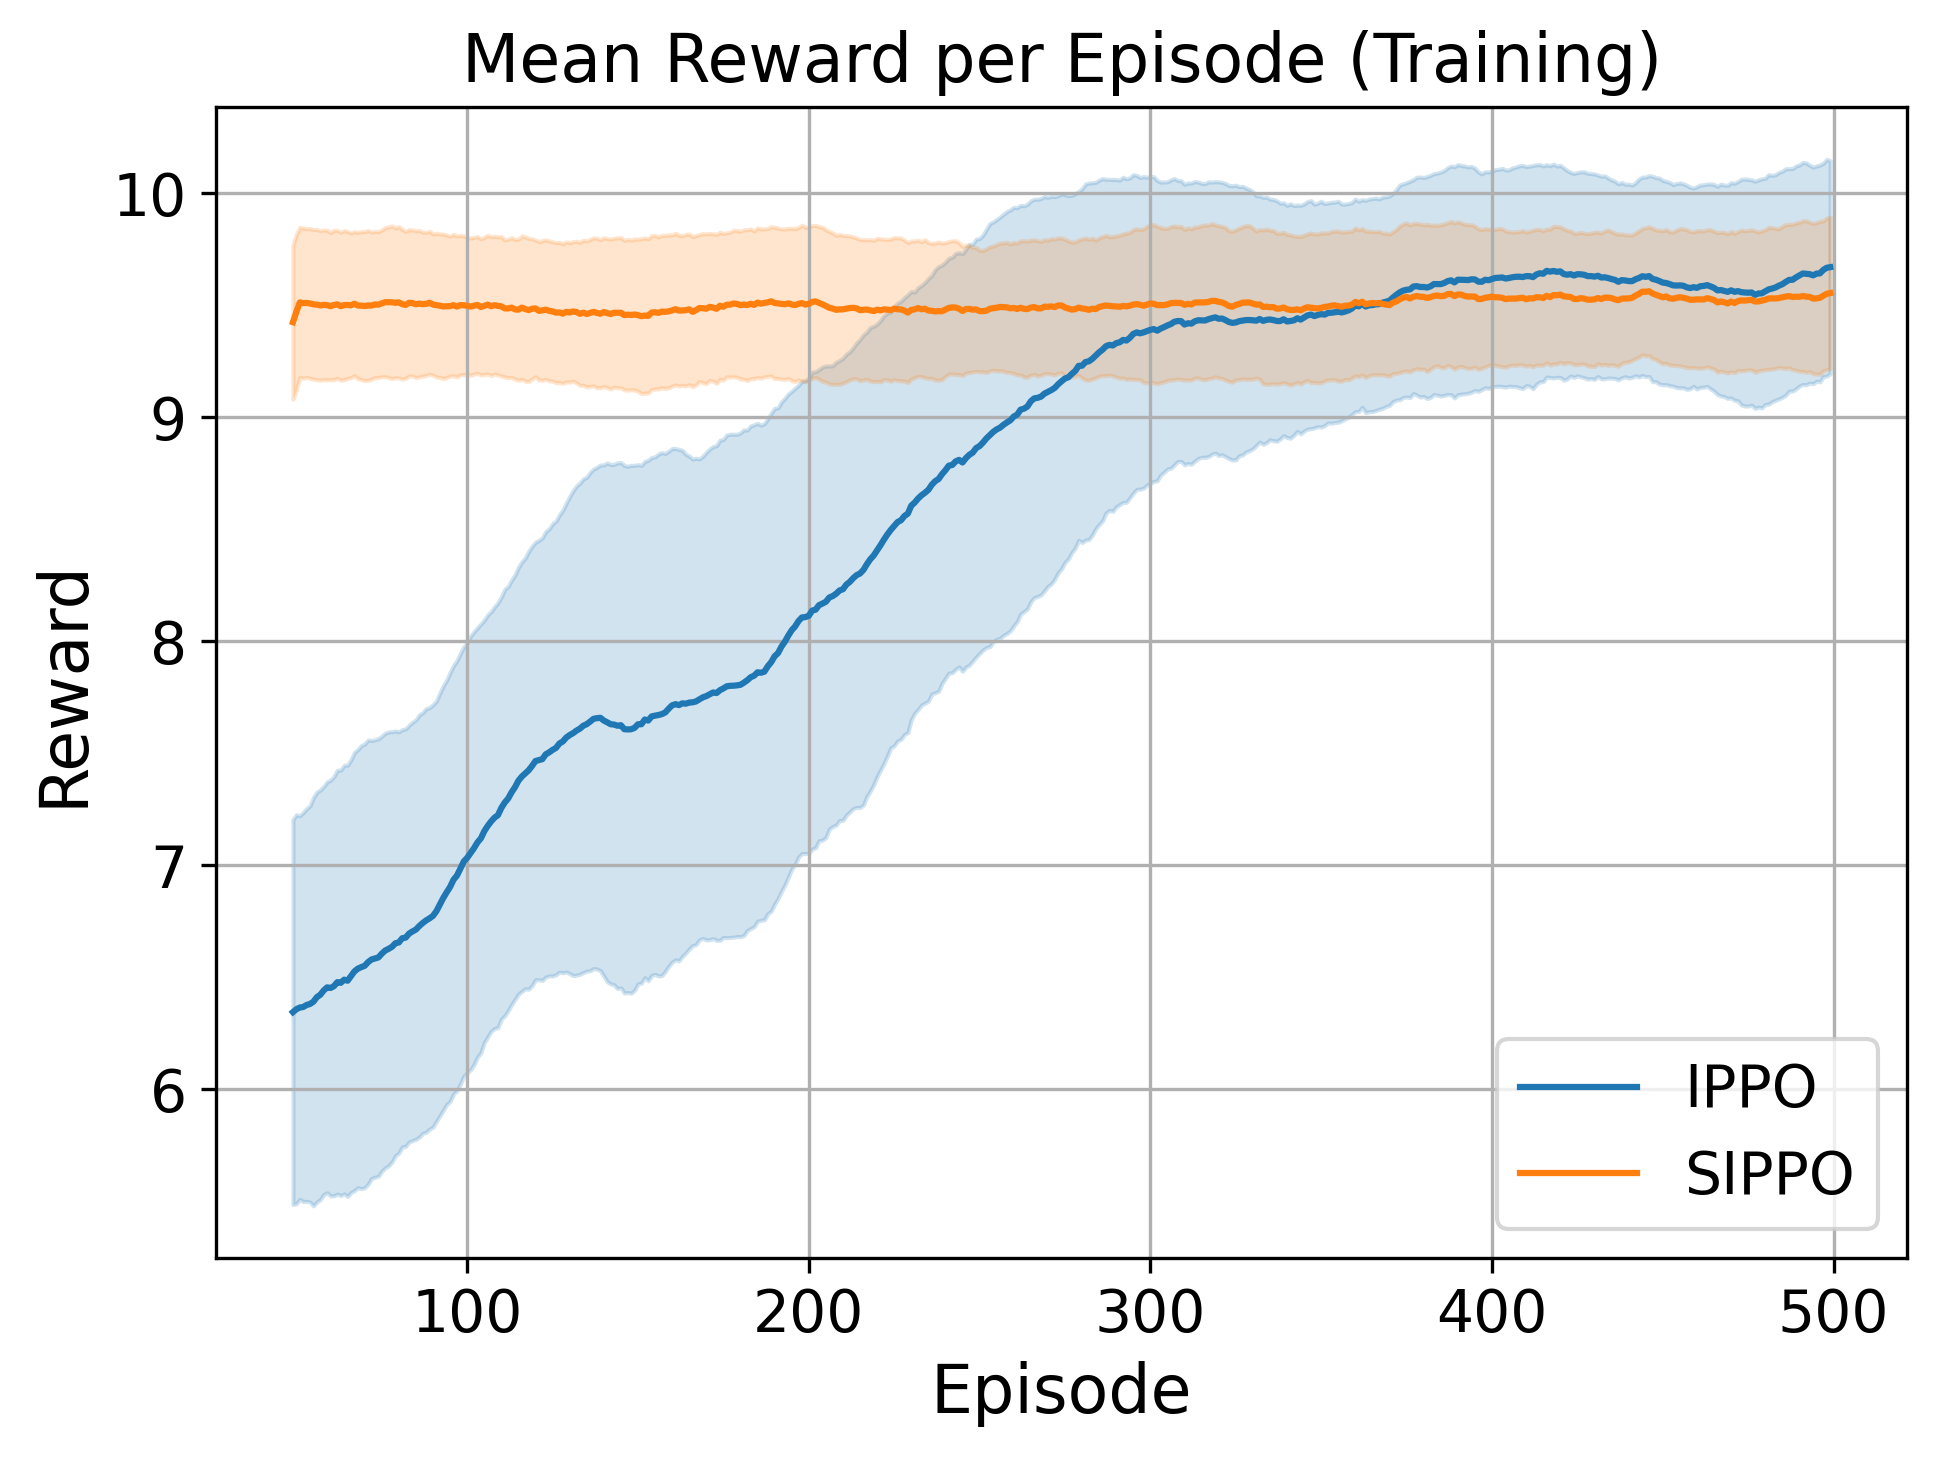
\includegraphics[width=0.9\textwidth]{Experiments/images/epgg/training_mu5_epgg.png}
        \vspace{0.3em}

        \textbf{(m)} Training ($\mu=5.0$)
        \label{fig:epgg_results:sub13}
    \end{minipage}
    \hfill
    \begin{minipage}[b]{0.3\textwidth}
        \centering
        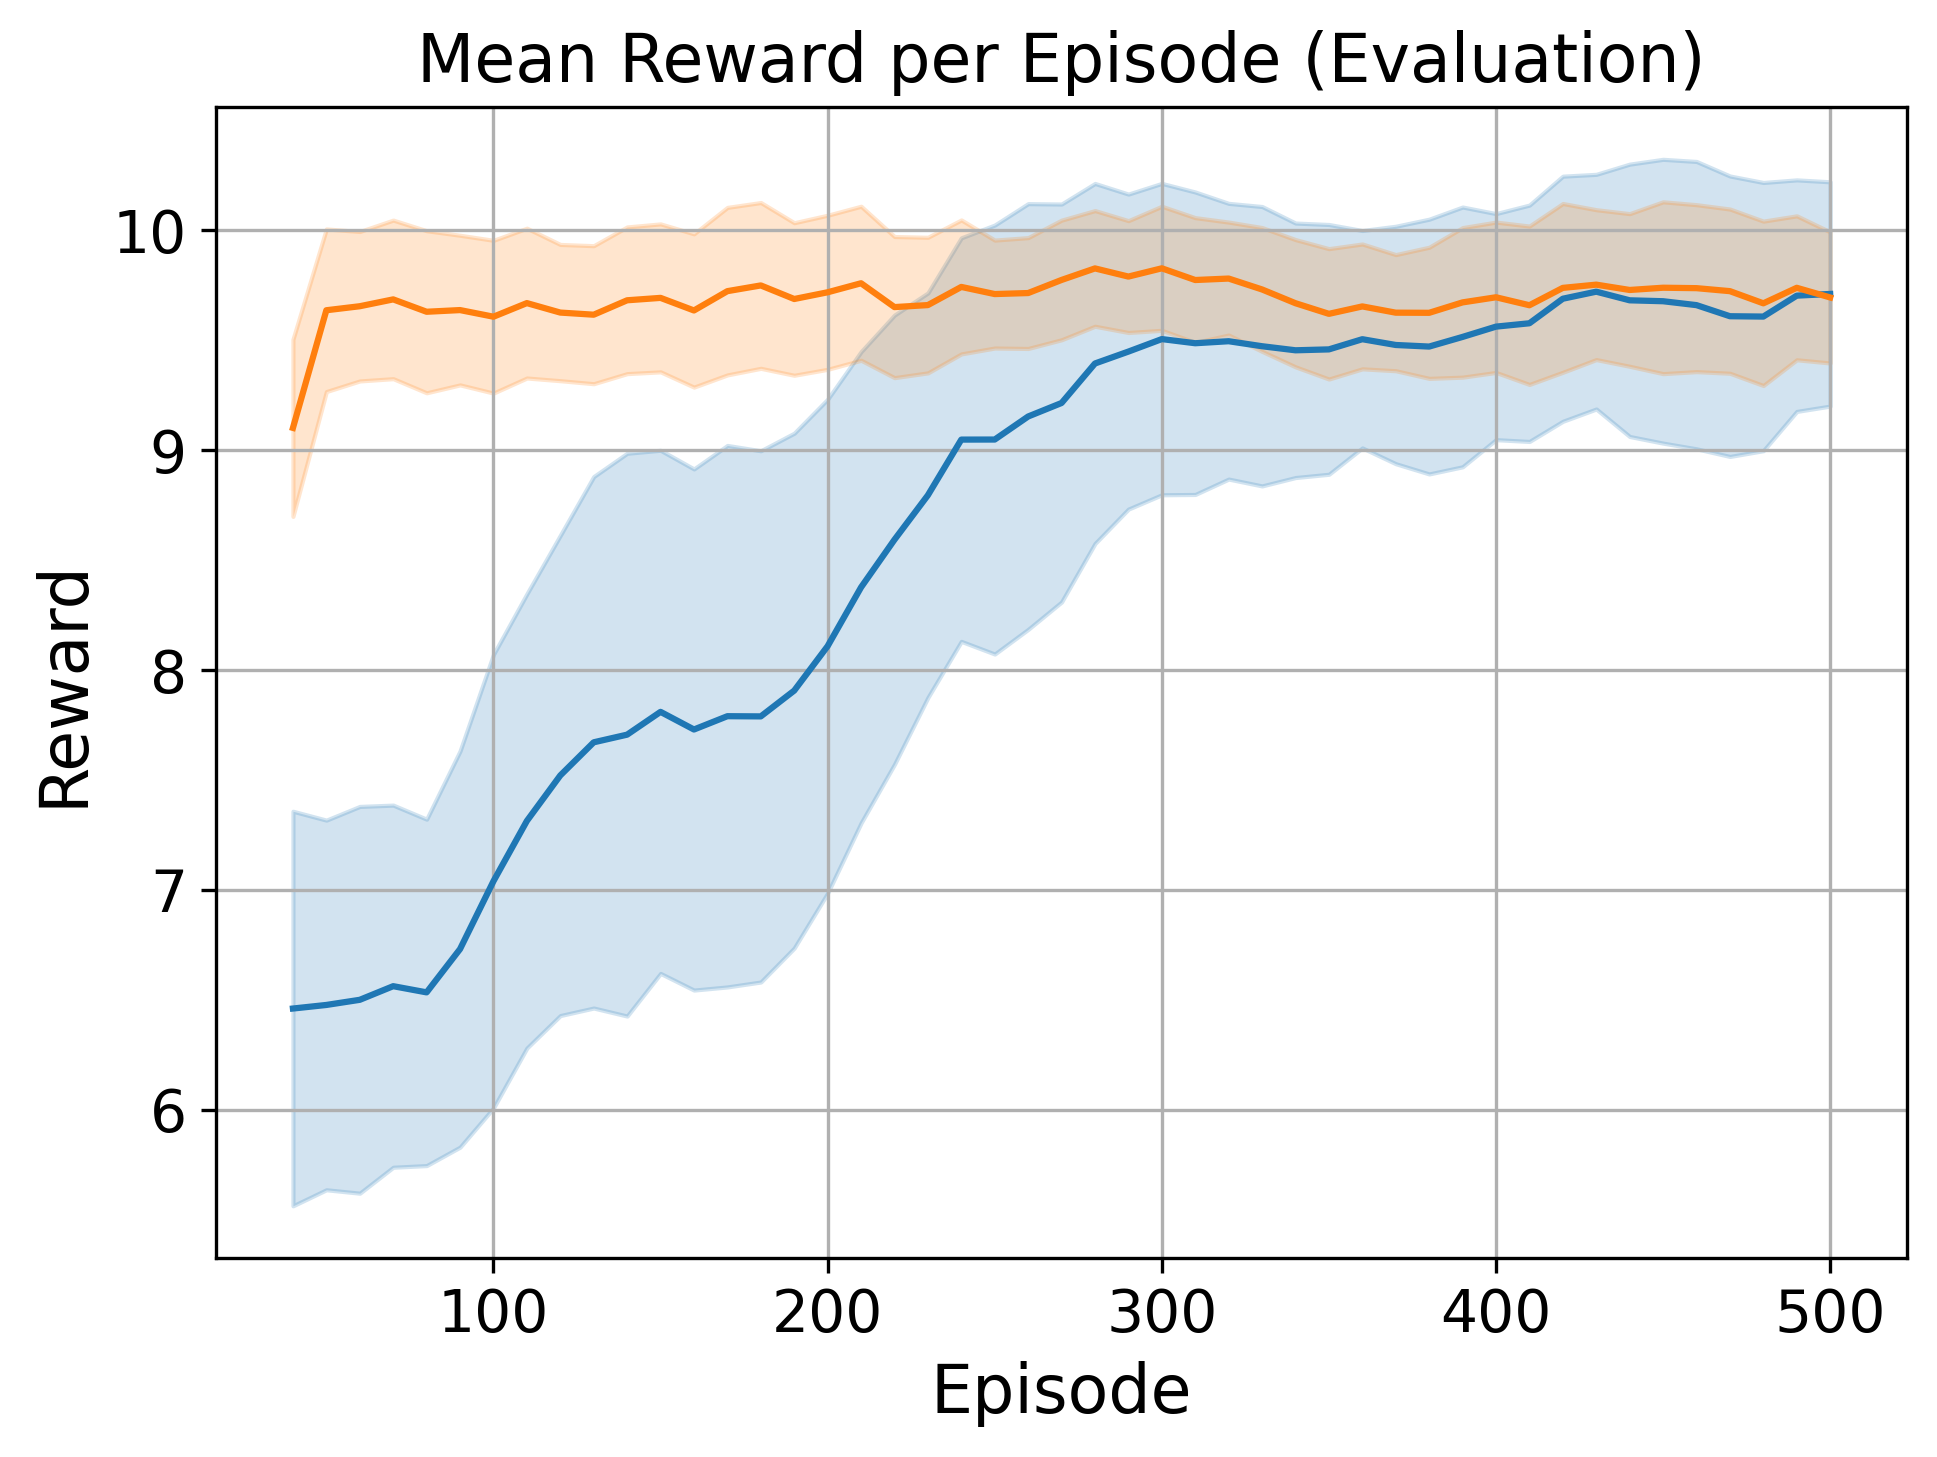
\includegraphics[width=0.9\textwidth]{Experiments/images/epgg/eval_mu5_epgg.png}
        \vspace{0.3em}

        \textbf{(n)} Evaluation ($\mu=5.0$)
        \label{fig:epgg_results:sub14}
    \end{minipage}
    \hfill
    \begin{minipage}[b]{0.3\textwidth}
        \centering
        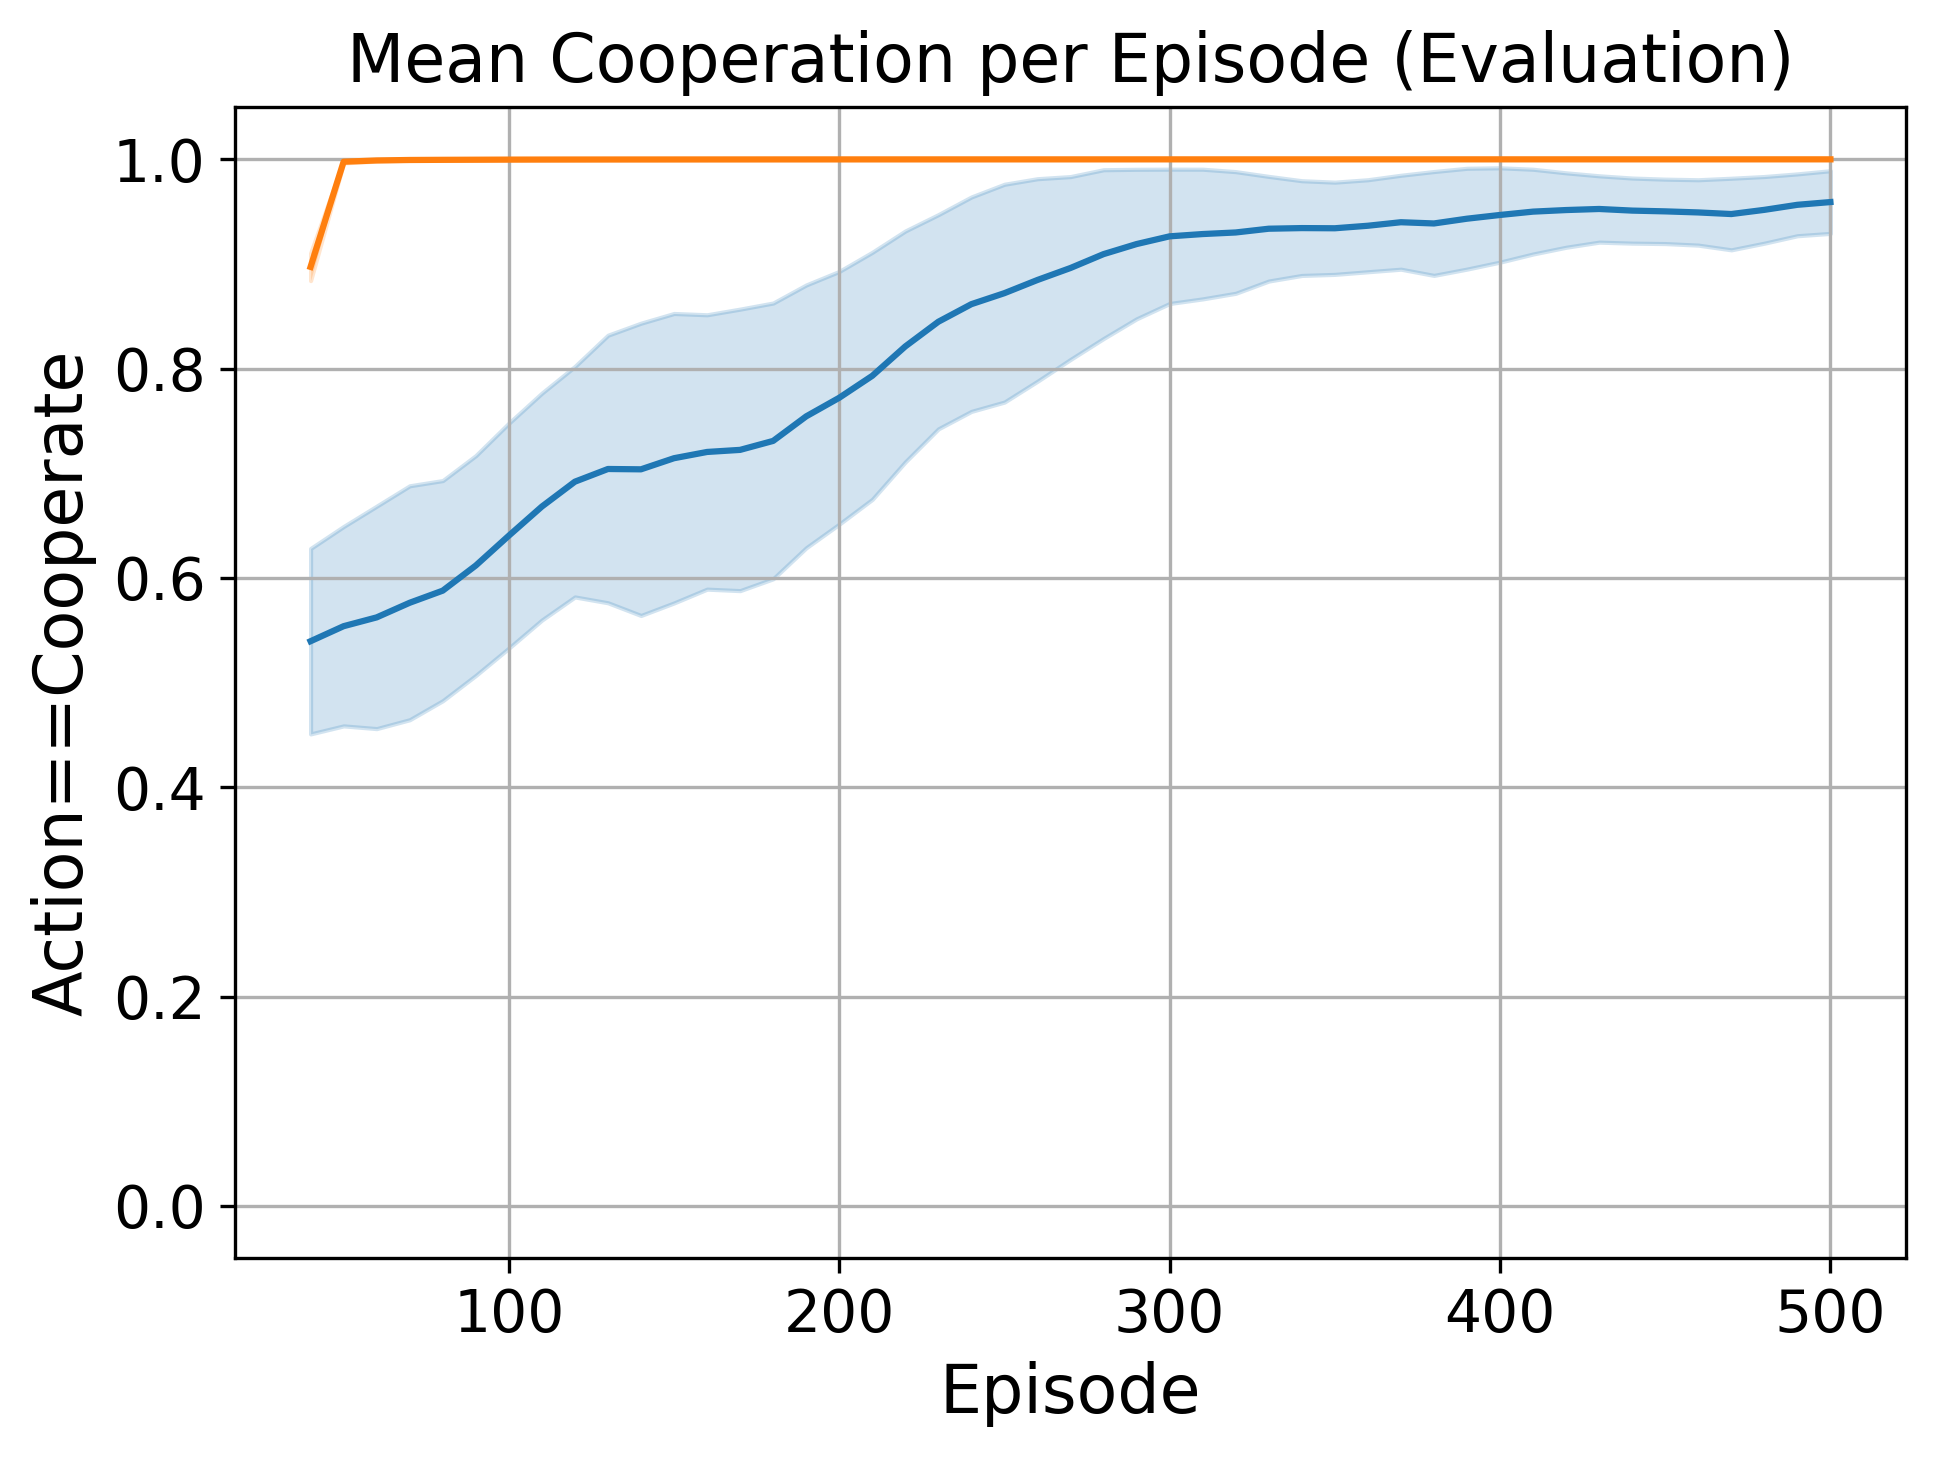
\includegraphics[width=0.9\textwidth]{Experiments/images/epgg/safety_mu5_epgg.png}
        \vspace{0.3em}

        \textbf{(o)} Safety ($\mu=5.0$)
        \label{fig:epgg_results:sub15}
    \end{minipage}

    \caption[Results for 2-player \textit{Extended Public Goods Game}.]{Training, evaluation, and safety results for the two-player EPGG for PLPG-based agents. The multiplicative factor $f_t$ is sampled from $\mathcal{N}(\mu,1)$, where $\mu \in \{0.5, 1.0, 1.5, 2.5, 5.0\}$ for different experiments. The lines represent the mean and the shadow the standard deviation over 5 seeds. Results are smoothed using a rolling average with window size 50.}
    \label{fig:epgg_results}
\end{figure*}